% !TeX spellcheck = en_US

\documentclass[twoside,11pt]{article}

% mathematics
\usepackage{amsmath,amssymb,amsthm}
\usepackage[abbrvbib,preprint]{jmlr2e}

% language and encoding
\usepackage[american]{babel} % American English
\usepackage[utf8x]{inputenc}
\usepackage{hyperref} % hyperlinks
  \hypersetup{hidelinks}
\pdfminorversion=7

\usepackage[capitalize,noabbrev]{cleveref}
  \creflabelformat{equation}{#2#1#3}
\theoremstyle{definition}
\newtheorem{defn}{Definition}
\newtheorem{exmp}{Example}
\newtheorem{prop}{Property}
\newtheorem{remk}{Remark}

% other packages
\usepackage{algorithmicx}
\usepackage{csquotes,natbib,url}
\usepackage{booktabs,graphicx,siunitx,tikz}
\usepackage[figuresright]{rotating}
\newcommand{\euro}{Euro}

% to format tab head differently from numeric body columns
\newcommand{\head}[1]{\multicolumn{1}{c}{#1}}

\sloppy
\frenchspacing

%\jmlrheading{1}{2023}{PAGES}{04/23}{PUBLISHED}{meila00a}{Marina Meil\u{a} and Michael I. Jordan}
\ShortHeadings{The Power of Linear Recurrent Neural Networks}{Stolzenburg, Litz, Michael, Obst}
\firstpageno{1}

\begin{document}

\title{The Power of Linear Recurrent Neural Networks}
\author{\name Frieder Stolzenburg \email fstolzenburg@hs-harz.de\\ %\orcid 0000-0002-4037-2445
	\name Sandra Litz\\ %\email litz\_sandra@web.de} \orcid 0009-0000-8147-4424
	\addr Department of Automation and Computer Sciences,
	Harz University of Applied Sciences,
	38855 Wernigerode, Germany
\AND	
	\name Olivia Michael\\ %\email olivia\_michael@hotmail.com \orcid 0000-0002-5719-2299
	\name Oliver Obst \email o.obst@westernsydney.edu.au\\ %\orcid 0000-0002-8284-2062
	\addr Centre for Research in Mathematics and Data Science,
	Western Sydney University,
	Penrith NSW 2751, Australia}
\editor{}
\maketitle

\begin{abstract}
Recurrent neural networks are a powerful means to cope with time series. We show
how autoregressive linear, i.e., linearly activated recurrent neural networks (LRNNs) can
approximate any time-dependent function $f(t)$ given by a number of function
values. The approximation can effectively be learned by simply solving a linear
equation system; no backpropagation or similar methods are needed. Furthermore,
and this is probably the main contribution of this article, the size of an
LRNN can be reduced significantly in one step after inspecting the spectrum
of the network transition matrix, i.e., its eigenvalues, by taking only the most
relevant components. Therefore, in contrast to other approaches, we do not only
learn network weights but also the network architecture. LRNNs have interesting
properties: They end up in ellipse trajectories in the long run and allow the
prediction of further values and compact representations of functions. We
demonstrate this by several experiments, among them multiple superimposed
oscillators (MSO), robotic soccer, and predicting stock prices. LRNNs outperform
the previous state-of-the-art for the MSO task with a minimal number of units.

\smallskip
\begin{keywords}
recurrent neural network; linear activation; time-series analysis; prediction;
dimensionality reduction; approximation theorem; ellipse trajectories.
\end{keywords}

\smallskip
\noindent\textbf{MSC class:} 15A06 \;$\cdot$\; \textbf{ACM class:} I.2.6%
\end{abstract}

\section{Introduction}

Deep learning in general means a class of machine learning algorithms that use a
cascade of multiple layers of nonlinear processing units for feature extraction
and transformation \citep{DY14}. The tremendous success of deep learning in
diverse fields of artificial intelligence, such as computer vision and natural
language processing, seems to depend on a bunch of ingredients: artificial,
possibly recurrent neural networks (RNNs), with nonlinearly activated neurons,
convolutional layers, and iterative training methods like backpropagation
\citep{GBC16}. But which of these components are really essential for machine
learning tasks such as time-series analysis?

Research in time series analysis and hence modeling dynamics of complex systems
has a long tradition and is still highly active due to its crucial role in many
real-world applications \citep{LBE15} like weather forecast, stock quotations,
comprehension of trajectories of objects and agents, or solving number puzzles
\citep{RK11,GW13}. The analysis of time series allows, among others, data
compression, i.e., compact representation of time series, e.g., by a function
$f(t)$, and prediction of further values.

Numerous research addresses these topics by RNNs, in particular variants of
networks with long short-term memory (LSTM) \citep{HS97}. In the following, we
consider an alternative, simple but very powerful type of RNNs: linear
recurrent neural networks (LRNNs). Thus we only use linear activation, which
allows us to minimize the network size in one step, namely by inspecting the
eigenvalues of the network transition matrix (cf. \cref{reduce}). Therefore, in
contrast to other approaches, we do not only learn network weights but also the
network architecture.

The rest of this paper is structured as follows: First, we briefly review related
works (\cref{related}). We then formally introduce LRNNs as a special and simple
kind of RNNs together with their properties, including the general network
dynamics and their long-term behavior (\cref{define}). Afterwards, learning
LRNNs is explained (\cref{learn}). It is a relatively straightforward procedure
which allows network size reduction; no backpropagation or gradient-descent
method is needed. We then discuss results and experiments (\cref{result}),
before we end up with conclusions (\cref{conclude}).

Interestingly, several results for LRNNs we present here can be achieved by
applying linear algebra and matrix analysis. Nonetheless, to the best of our
knowledge, the main contributions of this article have not been presented
before, namely that LRNNs can effectively be learned by a simple procedure and,
even more, their size can be reduced significantly in one step (cf.
\cref{learn}). In addition, the empirical evaluations of, in particular, the MSO
benchmark and stock price prediction (cf. \cref{mso,stock}) with LRNNs and other
approaches, e.g., LSTM networks, demonstrate the usefulness of our approach. We
therefore hope that several interested communities can profit from this work,
such as the neural engineering community, the time series prediction community,
and the ESN community.

\section{Related Works}\label{related}

\subsection{Echo State Networks}

Echo state networks (ESNs) \citep{JH04,Jae07} play a significant role in RNN
research as they provide an architecture and supervised learning principle for
RNNs. They do so by driving a random, large, fixed RNN, called \emph{reservoir}
in this context, with the input signal which then induces in each neuron within
this reservoir network a nonlinear response signal. They combine a desired
output signal by a trainable linear combination of all response signals,
allowing dimensionality reduction by so-called \emph{conceptors} \citep{Jae14,Jae17}.

\citet{XYH07} propose a variant of ESNs that work with several independent
(decoupled) smaller networks. ESN-style (random) initialization has been shown
effective for training RNNs with Hessian-free optimization~\citep{MS11}. The
latter paper addresses the problem of how to effectively train recurrent neural
networks on complex and difficult sequence modeling problems which may contain
long-term data dependencies. This can also be done with LRNNs (cf. MSO
benchmark, \cref{mso}).
\citet{Tin18} considers the effect of weight changes in linear symmetric ESNs on
(Fisher) memory of the network. Furthermore, from a solely theoretical point of view,
\citet{CW+16} investigate the asymptotic performance of linear ESNs.

\subsection{Recurrent Neural Networks}

Simple RNNs are proposed by \citet{Elm90}. By allowing them to accept sequences
as inputs and outputs rather than individual observations, RNNs extend the
standard feedforward multilayer perceptron networks. As shown in many sequence
modeling tasks, data points such as video frames, audio snippets, and sentence
segments are usually highly related in time. This results in RNNs being used as
the indispensable tools for modeling such temporal dependencies. Linear RNNs and
some of their properties (like short-term memory) are already investigated by
\citet{WLS94}. Unfortunately, however, it can be a struggle to train RNNs to
capture long-term dependencies \citep{BSF94,PMB13}. This is due to the
gradients vanishing or exploding during backpropagation which in turn makes the
gradient-based optimization difficult.

Nowadays, probably the most prominent and dominant type of RNNs are long
short-term memory (LSTM) networks introduced by \citet{HS97}. The expression \enquote{long
short-term} refers to the fact that LSTM is a model for the short-term memory
which can last for a long period of time. An LSTM is well-suited to classify,
process and predict time series given time lags of unknown size. They were
developed to deal with the exploding and vanishing gradient problem when
training traditional RNNs (see above). A common LSTM unit is composed of a cell,
an input gate, an output gate, and a forget gate. Each unit type is activated in
a different manner, whereas in this paper we consider completely linearly
activated RNNs.

\citet{OTC15} suggest to use the \enquote{NoBackTrack} algorithm in RNNs to
train its parameters. This algorithm works in an online, memoryless setting
which therefore requires no backpropagation through time. It is also scalable,
thus avoiding the large computational and memory cost of maintaining the full
gradient of the current state with respect to the parameters, but it still uses
an iterative method, namely gradient descent. In contrast to this and other
related works, in this paper we present a method working with linearly activated
RNNs that does not require backpropagation or similar procedures in the learning
phase.

\citet{HQ17} propose a novel state-frequency memory (SFM) RNN,
which aims to model the frequency patterns of the temporal sequences.
The key idea of the SFM is to decompose the memory states into different
frequency states. In doing so, they can explicitly learn the dependencies of
both the low and high frequency patterns. As we will see (cf. \cref{mso}),
RNNs in general can easily learn time series that have a constant frequency
spectrum which may be obtained also by Fourier analysis.

\citet{VKE19} propose a memory cell for recurrent neural networks that maintains
information across long windows of time using relatively few resources, called
Legendre memory unit (LMU). It is derived from the linear transfer function for
a continuous-time history of its input signal across a sliding window,
approximated by coupled differential equations, which can implicitly also be
solved by LRNNs (cf. \cref{rem}).
\citet{CSB21} propose an approach to address memorization challenges in RNNs
which puts forward a way between the random encoding in the reservoir paradigm
and the vanishing-gradient prone approach of fully-trained RNNs. The objective
is to train memorization units to maximize their short-term memory capacity,
employing linear autoencoder for sequences. In both cases, backpropagation is
employed, which is not needed for LRNNs whose network size is reduced
significantly in addition (cf. \cref{reduce}), thus we address the topic of
architecture learning.

Architecture learning, in particular the pruning of neural networks, has been
studied extensively in the literature. An early survey on pruning algorithms
for neural networks is given by \citet{Ree93}. In more recent work,
\citet{LAT19} present a method that prunes irrelevant connections between
neurons for a given task prior to training and is applicable to a variety of
modern neural network models, resulting in sparse networks. Furthermore,
\citet{MM+19} propose a method that estimates the contribution of a neuron to
the final loss and iteratively removes those with smaller scores. In contrast to
this, for LRNNs, the network architecture and hence its size is reduced in one
step by analyzing the network transition matrix (cf. \cref{reduce}).

\subsection{Autoregression}\label{regress}

An \emph{autoregressive model} is a representation of a type of random process
\citep{Aka69}. It specifies that the output variable or a vector thereof depends
linearly on its own previous values and on a stochastic term (white noise). In
consequence, the model is in the form of a stochastic differential equation as in
general (physical) dynamic systems \citep{CK14}. An LRNN is also linearly
activated, but its output does not only depend on its own previous values and
possibly white noise but on the complete state of the possibly big reservoir
whose dynamics is explicitly dealt with. In addition, the size of the network
might be reduced in the subsequent process. We will continue the comparison
between autoregression and LRNNs later (cf. \cref{output}) and mainly consider
autoregressive tasks in the following.

A popular choice in this context is the autoregressive integrated moving average
(ARIMA) model \citep{HK08,HA13}. A standard ARIMA($p,d,q$) model consists of
autoregression AR($p$) and a moving average MA($q$). The parameter $p$ describes
the history length (lag order) used to predict the time series at time $t$. We
have $f(t) = c_1 f(t-1) + \dots + c_p f(t-p) + e_t$ where $c_1,\dots,c_p$ are
(real-valued) autocorrelation coefficients and $e_t$, the residuals, are
Gaussian white noise. In the moving average process MA($q$), the value $q$
specifies the number of past residuals considered for prediction. An underlying
trend of the time series is modeled by using a drift, i.e., a constant that extends
the term. This procedure is particularly well-suited for stationary time series.
Many time series, however, exhibit non-stationary behavior and thus require a
transformation to make them stationary. This is achieved by investigating the
derivatives of the series, with the order of this process given by the parameter
$d$.

Autoregressive frameworks are common in current machine-learning applications
like language modeling, e.g., in the generative pre-trained transformer GPT-3 and their successors,
by next word prediction \citep{BM+20}. The model applied in this context,
however, is very complex (175 billion parameters and more) and non-linear.
Related to autoregression is autoencoding of sequences. For this, \citet{PS14}
show that linear autoencoders can be used for pre-training of RNNs, while we
establish completely linear RNNs here. Furthermore, \citet{Spe06} gives an
exact closed-form solution for the weights of the linear autoencoder, which is
related to the approximation theorem for LRNNs (cf. \cref{approx}).

\section{Linear Recurrent Neural Networks}\label{define}

RNNs often host several types of neurons, each activated in a different manner
\citep{Elm90,HS97}. In contrast to this, we here simply understand a homogeneous
interconnected group of standard neurons as a (recurrent) neural network which may have
arbitrary loops, akin to biological neuronal networks. We adopt a \emph{discrete
time model}, i.e., input and output can be represented by a time series and is
processed stepwise by the network.

\begin{defn}[time series]
A \emph{time series} is a series of data points in $d$ dimensions
$S(0),\dots,S(n) \in \mathbb{R}^d$ where $d \ge 1$ and $n \ge 0$.
\end{defn}

\begin{defn}[recurrent neural network]
A \emph{recurrent neural network} (RNN) is a directed graph consisting of
altogether $N$ nodes, called \emph{neurons}. $x(t)$ denotes the
\emph{activation} of the neuron $x$ at (discrete) time $t$. We may distinguish
three groups of neurons (cf. \cref{net}):
\begin{itemize}
  \item $N^\mathrm{in}$ \emph{input} neurons (usually without incoming edges)
	whose activation is given by an external source, e.g., a time series,
  \item $N^\mathrm{out}$ \emph{output} neurons (usually without outgoing edges)
	whose activation represents some output function, and
  \item $N^\mathrm{res}$ \emph{reservoir} or \emph{hidden} neurons (arbitrarily
	connected) that are used for auxiliary computations.
\end{itemize}
The sets of input and output neurons are not necessarily disjoint, they may even
be identical (cf. \cref{thedef}). Therefore, in the following, let
$N^\mathrm{in\,out}$ denote the overall number of neurons in the union of both
sets. Obviously it holds $N = N^\mathrm{in\,out}+N^\mathrm{res}$ and
$N^\mathrm{in\,out} \le N^\mathrm{in}+N^\mathrm{out}$.

The edges of the directed graph represent the network connections. They are
annotated with \emph{weights} which are compiled in the \emph{transition matrix}
$W$ of size $N \times N$. An entry~$w_{ij}$ in row~$i$ and column~$j$ denotes the weight of the edge
from neuron~$j$ to neuron~$i$. If there is no connection, then
$w_{ij} = 0$. The transition matrix has the form
\begin{equation}\label{matrix}
  W = \left[ \begin{array}{cc}
  \multicolumn{2}{c}{W^\mathrm{out}}\\
  W^\mathrm{in} & W^\mathrm{res}
\end{array} \right]
\end{equation}
containing the following weight matrices:
\begin{itemize}
  \item \emph{input} weights $W^\mathrm{in}$ (weights from the input and
	possibly the output to the reservoir, a matrix of size $N^\mathrm{res} \times N^\mathrm{in\,out}$),
  \item \emph{output} weights $W^\mathrm{out}$ (all weights to the output and
	possibly back to the input, a matrix of size $N^\mathrm{in\,out} \times N$), and
  \item \emph{reservoir} weights $W^\mathrm{res}$ (weights within the reservoir,
	a matrix of size $N^\mathrm{res} \times N^\mathrm{res}$).
\end{itemize}
\end{defn}

\begin{figure}
  \centering
  \usetikzlibrary {shapes.geometric}
\usetikzlibrary{positioning}
\begin{tikzpicture}[    
    node/.style={draw, circle, minimum size=0.8cm},
    arrow/.style={->, >=latex, thick},
    hidden_layer/.style={draw, ellipse, minimum width=7cm, minimum height=4.5cm}
]

% Input layer
\node[node, label={[label distance=0.5cm]north:Input}] (x1) at (0, 0) {$x_1$};
\node[node] (x2) at (0, -1.5) {$x_2$};
\node[node, label={[label distance=0.5cm]north east:$\mathbf{W}^\text{in}$}] (x3) at (0, -3) {$x_3$};

% Hidden layer
\node[hidden_layer, label={[label distance=0.5cm]north:Reservoir}] (hidden) at (5, -1.5) {};
\node[node] (h1) at (3, -1) {$h_1$};
\node[node] (h2) at (3.5, -2.5) {$h_2$};
\node[node] (h3) at (4.5, 0) {$h_3$};
\node[node] (h4) at (5.5, -1.5) {$h_4$};
\node[node] (h5) at (5, -3) {$h_5$};
\node[node, label={[label distance=0.3cm]north west:$\mathbf{W}^\text{res}$}] (h6) at (7, -1) {$h_6$};
\node[node] (h7) at (6.5, -2.7) {$h_7$};

% Output layer
\node[node, label={[label distance=0.5cm]north:Output}] (y1) at (10, -0.75) {$y_1$};
\node[node, label={[label distance=0.1cm]north west:$\mathbf{W}^\text{out}$}] (y2) at (10, -2.25) {$y_2$};

% Edges
\foreach \i in {1,2,3}
    \draw[arrow] (x\i) -- (hidden);

\foreach \j in {1,2}
    \draw[arrow] (hidden) -- (y\j);

% Recurrent connections
\draw[arrow, bend right] (h1) to[out=70,in=135,looseness=0.8] (h3);
\draw[arrow, bend right] (h1) to[out=110,in=135,looseness=0.8] (h5);
\draw[arrow, bend right] (h2) to[out=90,in=90,looseness=0.8] (h4);
\draw[arrow, bend right] (h3) to[out=40,in=160,looseness=0.8] (h7);
\draw[arrow, bend right] (h4) to[out=330,in=195,looseness=0.8] (h7);
\draw[arrow, bend right] (h5) to[out=0,in=200,looseness=0.8] (h6);
\draw[arrow, bend right] (h5) to[out=45,in=130,looseness=0.8] (h2);

\end{tikzpicture}

  \caption{General recurrent neural network. In ESNs, only output weights are
	trained and the hidden layer is also called reservoir.}
  \label{net}
\end{figure}

Let us now define the \emph{network activity}: The initial
configuration of the neural network is given by a column vector $s$ with $N$
components, called \emph{start vector}. It represents the network state at the
start time $t=t_0$. Because of the discrete time model, the activation
of a (non-input) neuron $x_i$ at time $t+\tau$ (for some time step $\tau>0$) from
the activation at time $t$ of the neurons $x_1,\dots,x_k$ (for some $k \ge 0$ ) that
are connected to $x_i$ with the weights $w_{i1},\dots,w_{ik}$ is computed as
follows:
\begin{equation}\label{recur}
	x_i(t+\tau) = g\big(w_{i1}\,x_1(t) +\dots+ w_{ik}\,x_k(t)\big)
\end{equation}
This has to be done simultaneously for all neurons of the network. Here $g$ is a
(real-valued) \emph{activation function}. Although we will not make use of it,
$g$ may be different for different parts of the network.
Usually, a nonlinear, bounded, strictly increasing sigmoidal function $g$ is
used, e.g., the logistic function, the hyperbolic tangent ($\tanh$), or the
softplus function \citep[Sect.~3.10]{GBC16}. In the following, we employ simply
the (linear) identity function and can still approximate arbitrary
time-dependent functions (cf. \cref{approx}).

\begin{defn}[linear recurrent neural network]\label{thedef}
A \emph{linear recurrent network} (LRNN) is an RNN with the
following properties:
\begin{enumerate}
  \item For the start time, it holds that $t_0=0$ and $\tau$ is constant, usually $\tau=1$.
  \item The initial state $S(0)$ of the given time series constitutes the first
	$d$ components of the start vector $s$.
  \item For all neurons we have \emph{linear activation}, i.e., everywhere $g$
	is the identity.
  \item The weights in $W^\mathrm{in}$ and $W^\mathrm{res}$ are taken
	randomly, independently, and identically distributed from the standard
	normal distribution, i.e., the Gaussian distribution with mean $\mu = 0$
	and standard deviation $\sigma = 1$, and remain unchanged all the time,
	whereas the output weights $W^\mathrm{out}$ are learned (cf. \cref{output}).
  \item The spectral radius of the reservoir weights matrix $W^\mathrm{res}$ is
	set to $1$, i.e., $W^\mathrm{res}$ is divided by the maximal absolute
	value of all its eigenvalues. Note that the spectral radius of the
	overall transition matrix $W$ may still be greater than $1$ if required
	by the application (cf. \cref{continued}).
  \item There is no distinction between input and output but only one (joint)
	group of $N^\mathrm{in\,out} = N^\mathrm{in}=N^\mathrm{out}=d$ input/output neurons. They may
	be arbitrarily connected like the reservoir neurons. We thus can imagine
	the whole network as a big reservoir because the input/output neurons
	are not particularly special.
\end{enumerate}
\end{defn}

LRNNs can run in one of two \emph{modes}: either receiving input or generating
(i.e., predicting) output. In output generating mode, the network runs
autonomously, thus without external input. In this case, \cref{recur} is applied
to all neurons including the input/output neurons. The output from the
previous time step is copied to the input. In input receiving mode, the
activation of every input/output neuron $x$ at time $t$ is always overwritten
with the respective input value at time $t$ given by the time series $S$.

\subsection{Examples}

\begin{exmp}\label{parabola}
The function $f(t) = t^2$ can be realized by an LRNN (in output generating mode)
with three neurons (cf. \cref{examples}\,a). The respective transition matrix
$W$ and start vector $s$ are:
\[ W = \left[ \begin{array}{ccc}
	1 & 2 & 1\\
	0 & 1 & 1\\
	0 & 0 & 1
   \end{array} \right]
   \text{~and~} s = \left[ \begin{array}{c}
	0\\
	0\\
	1
   \end{array} \right]
\]
Consequently, starting at $t=0$ with time step $\tau=1$, we have:
\begin{itemize}
  \item $x_3(0) = 1$, $x_3(t+1) = x_3(t)$, and hence $x_3(t)=1$ in general.
  \item $x_2(0) = 0$, $x_2(t+1) = x_2(t)+x_3(t) = x_2(t)+1$, and hence $x_2(t)=t$.
  \item $x_1(0) = 0$, $x_1(t+1) = x_1(t)+ 2\,x_2(t) + x_3(t) = x_1(t)+ 2\,t +
	1$, and hence $x_1(t) = t^2$ because of the identity $(t+1)^2 = t^2 +
	2\,t + 1$ (cf. first row of the transition matrix $W$).
\end{itemize}
Thus, in the neuron $x_1$, the function $f(t)$ is computed. It is the only
input/output neuron.
\end{exmp}

\begin{exmp}\label{fibonacci}
The Fibonacci series ($0,1,1,2,3,5,8,\dots$) can be defined as follows:
\[ f(t) = \left\{ \begin{array}{ll}
	t, & t=0,1\\
	f(t-1)+f(t-2), & \text{otherwise}
\end{array} \right. \]
It can be realized by an LRNN (in output generating mode) with just two neurons
(cf. \cref{examples}\,b). The respective transition matrix $W$ and start vector
$s$ can be directly derived from the recursive definition of $f$:
\[ W = \left[ \begin{array}{cc}
	0 & 1\\
	1 & 1
   \end{array} \right]
   \text{~and~} s = \left[ \begin{array}{c}
	0\\
	1
   \end{array} \right]
\]
Again, the function $f(t)$ is computed in the only input/output neuron $x_1$. In
the other neuron $x_2$, $f(t+1)$ is generated. There is a closed-form expression
for the Fibonacci series, revealing its exponential growth, known as
\emph{Binet's formula}:
\begin{equation}\label{binet}
   f(t) = \frac{{\lambda_1}^t-{\lambda_2}^t}{\sqrt{5}}
	\text{~with~} \lambda_1 = \displaystyle\frac{1+\sqrt{5}}{2} \approx 1.6803
	\text{~(golden ratio) and~} \lambda_2 = 1-\lambda_1
\end{equation}
Interestingly, $\lambda_1$ and $\lambda_2$ are the eigenvalues of the transition
matrix $W$. Furthermore, Binet's formula can be used to create another LRNN to
calculate the Fibonacci series (cf. \cref{examples}\,c). We will come back to
this later (in \cref{continued}).
\end{exmp}

\begin{figure}
  \begin{minipage}[t]{0.3\textwidth}
	(a) 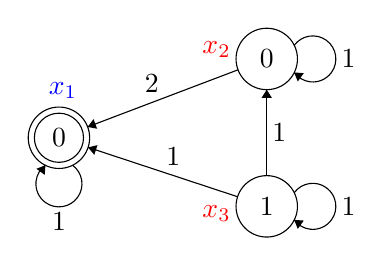
\begin{tikzpicture}[scale=0.13]
\tikzstyle{every node}+=[inner sep=0pt]
\draw [blue] (5,-25) node {$x_1$};
\draw [red] (20,-21) node {$x_2$};
\draw [red] (20,-37) node {$x_3$};
\draw [black] (4.6,-29.6) circle (3);
\draw (4.6,-29.6) node {$0$};
\draw [black] (4.6,-29.6) circle (2.4);
\draw [black] (24.9,-21.9) circle (3);
\draw (24.9,-21.9) node {$0$};
\draw [black] (24.9,-36.3) circle (3);
\draw (24.9,-36.3) node {$1$};
\draw [black] (24.9,-33.3) -- (24.9,-24.9);
\fill [black] (24.9,-24.9) -- (24.4,-25.7) -- (25.4,-25.7);
\draw (25.4,-29.1) node [right] {$1$};
\draw [black] (27.58,-20.577) arc (144:-144:2.25);
\draw (32.15,-21.9) node [right] {$1$};
\fill [black] (27.58,-23.22) -- (27.93,-24.1) -- (28.52,-23.29);
\draw [black] (27.58,-34.977) arc (144:-144:2.25);
\draw (32.15,-36.3) node [right] {$1$};
\fill [black] (27.58,-37.62) -- (27.93,-38.5) -- (28.52,-37.69);
\draw [black] (22.1,-22.96) -- (7.4,-28.54);
\fill [black] (7.4,-28.54) -- (8.33,-28.72) -- (7.98,-27.78);
\draw (13.68,-25.22) node [above] {$2$};
\draw [black] (22.05,-35.36) -- (7.45,-30.54);
\fill [black] (7.45,-30.54) -- (8.05,-31.27) -- (8.37,-30.32);
\draw (15.76,-32.41) node [above] {$1$};
\draw [black] (5.923,-32.28) arc (54:-234:2.25);
\draw (4.6,-36.85) node [below] {$1$};
\fill [black] (3.28,-32.28) -- (2.4,-32.63) -- (3.21,-33.22);
\end{tikzpicture}


  \end{minipage}
	\hfill
  \begin{minipage}[t]{0.3\textwidth}
	(b) 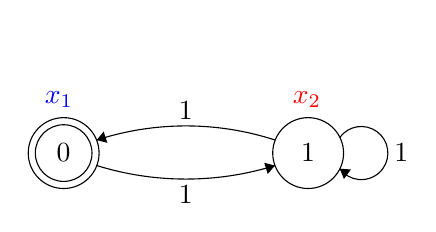
\begin{tikzpicture}[scale=0.15]
\tikzstyle{every node}+=[inner sep=0pt]
\draw (4,-19) node {};
\draw [blue] (5,-25) node {$x_1$};
\draw [red] (26,-25) node {$x_2$};
\draw [black] (5.4,-29.5) circle (3);
\draw (5.4,-29.5) node {$0$};
\draw [black] (5.4,-29.5) circle (2.4);
\draw [black] (26.1,-29.5) circle (3);
\draw (26.1,-29.5) node {$1$};
\draw [black] (23.294,-30.557) arc (-72.74231:-107.25769:25.429);
\fill [black] (23.29,-30.56) -- (22.38,-30.32) -- (22.68,-31.27);
\draw (15.75,-32.2) node [below] {$1$};
\draw [black] (8.189,-28.399) arc (108.02845:71.97155:24.432);
\fill [black] (8.19,-28.4) -- (9.1,-28.63) -- (8.79,-27.68);
\draw (15.75,-26.7) node [above] {$1$};
\draw [black] (28.78,-28.177) arc (144:-144:2.25);
\draw (33.35,-29.5) node [right] {$1$};
\fill [black] (28.78,-30.82) -- (29.13,-31.7) -- (29.72,-30.89);
\end{tikzpicture}


  \end{minipage}
	\hfill
  \begin{minipage}[t]{0.34\textwidth}
	(c) 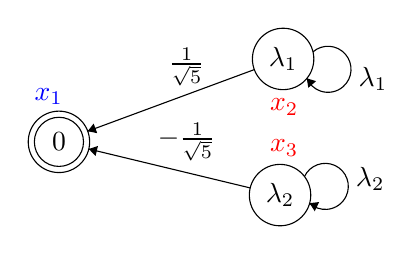
\begin{tikzpicture}[scale=0.13]
\tikzstyle{every node}+=[inner sep=0pt]
\draw [blue] (5,-7) node {$x_1$};
\draw [red] (28,-8) node {$x_2$};
\draw [red] (28,-12) node {$x_3$};
\draw [black] (6,-11.4) circle (3);
\draw (6,-11.4) node {$0$};
\draw [black] (6,-11.4) circle (2.4);
\draw [black] (27.9,-3.3) circle (3);
\draw (27.9,-3.3) node {$\lambda_1$};
\draw [black] (27.6,-16.6) circle (3);
\draw (27.6,-16.6) node {$\lambda_2$};
\draw [black] (25.09,-4.34) -- (8.81,-10.36);
\fill [black] (8.81,-10.36) -- (9.74,-10.55) -- (9.39,-9.61);
\draw (18.47,-6.00) node [above] {$\frac{1}{\sqrt{5}}$};
\draw [black] (30.808,-2.614) arc (131.00538:-156.99462:2.25);
\draw (35.23,-5.22) node [right] {$\lambda_1$};
\fill [black] (30.21,-5.19) -- (30.36,-6.12) -- (31.12,-5.47);
\draw [black] (29.982,-14.795) arc (154.88553:-133.11447:2.25);
\draw (34.96,-15.03) node [right] {$\lambda_2$};
\fill [black] (30.48,-17.39) -- (30.99,-18.18) -- (31.42,-17.28);
\draw [black] (24.68,-15.9) -- (8.92,-12.1);
\fill [black] (8.92,-12.1) -- (9.58,-12.78) -- (9.81,-11.8);
\draw (18.47,-13.32) node [above] {$-\frac{1}{\sqrt{5}}$};
\end{tikzpicture}


  \end{minipage}
  \caption{LRNNs for (a) $f(t) = t^2$ and (b\,+\,c) the Fibonacci series
	($0,1,1,2,3,5,8,\dots$) with time step $\tau=1$. In each case, the input/output neuron
	$x_1$ is marked by a double circle. The initial values of the neurons at
	time $t_0=0$ are written in the nodes. The weights are annotated at the
	edges.}
  \label{examples}
\end{figure}

\begin{remk}\label{rem}
LRNNs are well suited to represent differential equations and to solve them
numerically. To see this, consider the homogeneous linear differential equation
\begin{equation}
	\sum_{k=0}^n c_k\,x^{(k)}(t) = 0 \label{diff}
\end{equation}
where $c_k \in \mathbb{R}$ are constant coefficients with $c_n \neq 0$,
$x^{(k)}(t)$ is the $k$-th derivative of the function $x$ with respect to time
$t$, and $n>0$. For a function $x$ and its first derivative $\dot{x}$ with
respect to time $t$, we have
\begin{equation}
  \dot{x}(t) = \lim\limits_{\tau \to 0} \frac{x(t+\tau)-x(t)}{\tau}
	\quad\text{and hence}\quad
  x(t+\tau) \approx x(t) + \tau\,\dot{x}(t) \label{limit}
\end{equation}
for small time steps $\tau>0$. If we consider the difference of \cref{diff}
between the times $t+\tau$ and $t$ divided by $\tau$ we obtain by applying
\cref{limit} to $x^{(k)}(t)$ for $k \ge 0$:
\begin{eqnarray*}
  0 & = & \frac{\displaystyle\sum_{k=0}^n c_k\,x^{(k)}(t+\tau)-\sum_{k=0}^n c_k\,x^{(k)}(t)}{\tau}\\
    & = & \sum_{k=0}^{n-1} c_k \frac{x^{(k)}(t+\tau)-x^{(k)}(t)}{\tau} + c_n \frac{x^{(n)}(t+\tau)-x^{(n)}(t)}{\tau}\\
    & \approx & \sum_{k=0}^{n-1} c_k\,x^{(k+1)}(t) + \frac{c_n}{\tau} \left(x^{(n)}(t+\tau)-x^{(n)}(t)\right)
\end{eqnarray*}
This is equivalent to:
\[
	x^{(n)}(t+\tau)
	\approx x^{(n)}(t) - \frac{\tau}{c_n}\,\sum_{k=0}^{n-1} c_k\,x^{(k+1)}(t)
\]
Therefore, we can solve differential equations approximately by LRNNs with
start vector $s$, which should satisfy \cref{diff}, and the following transition
matrix:
\[ W = \left[ \begin{array}{*{5}{c}}
	1 & \tau & 0 & \cdots & 0\\
	0 & 1 & \tau & \ddots & 0\\
	\vdots & \ddots & \ddots & \ddots & 0\\
	0 & \cdots & 0 & 1 & \tau\\
	0 & -\tau \frac{c_0}{c_n} & \cdots & -\tau \frac{c_{n-2}}{c_n} & 1\!-\!\tau \frac{c_{n-1}}{c_n}
\end{array} \right] \]
\end{remk}

\begin{exmp}\label{exp}
The exponential function $\exp(t) = e^t$ can be defined by the differential
equation $\dot{x}(t) = x(t)$, i.e., we have $c_0 = 1$ and $c_1 = -1$ in
\cref{diff}. In consequence, according to \cref{rem} and because of $\exp(0)=\dot{\exp}(0)=1$,
the transition matrix $W$ and start vector $s$ of the corresponding LRNN are:
\[ W = \left[ \begin{array}{cc}
	1 & \tau\\
	0 & 1\!+\!\tau
   \end{array} \right]
   \text{~and~} s = \left[ \begin{array}{c}
	1\\
	1
   \end{array} \right]
\]
Induction over time yields immediately $x(t) = \dot{x}(t) = (1+\tau)^{t/\tau}
\approx e^t$ for small $\tau>0$ (according to Euler) as expected.
\end{exmp}

The strong relationship between RNNs and differential equations is already known
\citep[Sect.~9]{KB+16} as well as the extraction of eigenvalues to describe
dynamical systems \citep[Sect.~5]{Str15}. Nevertheless, as we will show in the
rest of this paper, the combination of both provides an effective method for
network size reduction (cf. \cref{reduce}) and therefore seems to be worthwhile
to be considered by the machine learning community in more detail.

\subsection{Network Dynamics}\label{dynamics}

An LRNN runs through network states $f(t)$ for $t
\ge 0$. It holds (in output generating mode)
\[ f(t) = \left\{ \begin{array}{ll}
	s, & t=0\\
	W \cdot f(t-\tau), & \text{otherwise}
\end{array} \right. \]
and hence simply $f(t) = W^t \cdot s$. Note that we assume $\tau = 1$ here (cf. \cref{thedef}).

\begin{prop}\label{jordan}
Let $W = V \cdot J \cdot V^{-1}$ be the Jordan decomposition of the transition
matrix $W$ where $J$ is the direct sum of one or more Jordan blocks, i.e., a
block diagonal matrix formed of Jordan blocks
\[ J_m(\lambda) = \left[ \begin{array}{*{5}{c}}
  \lambda & 1 & 0 & \cdots & 0\\
  0 & \lambda & 1 & \ddots & \vdots\\
  \vdots & \ddots & \ddots & \ddots & 0\\
  \vdots & & \ddots & \lambda & 1\\
  0 & \cdots & \cdots & 0 & \lambda
\end{array} \right] \]
in general with different sizes $m \times m$ and different eigenvalues $\lambda$,
and $V$ is a matrix consisting of the corresponding eigen- and principal column vectors.
Then we have: \[ f(t) = W^t \cdot s = V \cdot J^t \cdot V^{-1} \cdot s \]

If we decompose $V$ into matrices $v$ of size $N \times m$ and the column vector
$V^{-1} \cdot s$ into a stack of column vectors $w$ of size $m$, corresponding
to the Jordan blocks in $J$, then $f(t)$ can be expressed as a sum of vectors $u
= v \cdot J_m(\lambda)^t \cdot w$ where the Jordan block powers are upper
triangular Toeplitz matrices, i.e., in which each descending diagonal from left
to right is constant, with:
\begin{equation}\label{power}
  \Big( J_m(\lambda)^t \Big)_{ij} = \binom{t}{j-i}\,\lambda^{t-(j-i)}
	\quad\text{\citep[Sect.~3.2.5]{HJ13}}
\end{equation}
\end{prop}

\begin{remk}\label{general}
Although the parameter $t$ is discrete, i.e., a nonnegative integer number, the
values of $f(t) = W^t \cdot s$ can also be computed for $t \in \mathbb{R}$ and
are always real. For this, we consider the Jordan block powers from \cref{power}:
\begin{itemize}
  \item The definition of the binomial coefficient $\binom{t}{k} =
	\frac{t\,(t-1)\,\cdots\,(t-k+1)}{k\,(k-1)\,\cdots\,1}$ is applicable for
	real and even complex $t$ and nonnegative integer $k$. For negative $k$,
	we have $\binom{t}{k} = 0$.
  \item For real matrices $W$, there are always complex conjugate eigenvalue
	pairs $\lambda$ and $\overline{\lambda}$ and corresponding complex
	coefficients $c$ and $\overline{c}$ (resulting from the vectors $u$ in
	\cref{jordan}). With $c = |c|\,e^{\mathfrak{i}\psi}$ and
	$\lambda = |\lambda|\,e^{\mathfrak{i}\omega}$, we get $c\,\lambda^t +
	\overline{c}\,\overline{\lambda}{}^t = |c|\,|\lambda|^t \cos(\omega
	t+\psi)$ applying Euler's formula. This obviously is defined for all
	$t \in \mathbb{R}$ and always yields real-valued $f(t)$.
  \item Negative real eigenvalues, i.e., the case $\lambda<0$, should be treated
	in a special way, namely by replacing $\lambda^t$ by $|\lambda|^t \cos(\pi t)$.
	Both terms coincide for integer $t$, but only the latter is real-valued
	for all $t \in \mathbb{R}$. The powers of positive real eigenvalues
	$\lambda$ are always positive and real and hence need no further consideration.
\end{itemize}
\end{remk}

A Jordan decomposition exists for every square matrix $W$ \citep[Theorem~3.1.11]{HJ13}.
But if $W$ has $N$ distinct eigenvectors, there is a simpler decomposition,
called \emph{eigendecomposition}. The transition matrix $W$ is
\emph{diagonalizable} in this case, i.e., similar to a diagonal matrix $D$, and
the network dynamics can be directly described by means of the eigenvalues and
eigenvectors of $W$:

\begin{prop}\label{eigen}
Let $W = V \cdot D \cdot V^{-1}$ be the eigendecomposition of the transition matrix $W$ with column
eigenvectors $v_1,\dots,v_N$ in $V$ and corresponding eigenvalues $\lambda_1, \dots, \lambda_N$,
on the diagonal of the diagonal matrix $D$, sorted in decreasing order with
respect to their absolute values. Like every column vector, we can represent the
start vector $s$ as linear combination of the eigenvectors, namely as $s =
x_1 v_1 + \dots + x_N v_N = V \cdot x$ where $x = \big[ x_1 \cdots x_N
\big]^\top$. It follows $x = V^{-1} \cdot s$.
Since $W$ is a linear mapping and for each eigenvector $v_k$ with eigenvalue
$\lambda_k$ with $1 \le k \le N$ it holds that $W \cdot v_k = \lambda_k\, v_k$, we
have $W \cdot s = W \cdot (x_1 v_1 + \dots + x_N v_N) = x_1 \lambda_1 v_1 +
\dots + x_N \lambda_N v_N$. Induction over $t$ yields immediately:
\begin{equation}\label{form}
	f(t) = W^t \cdot s = V \cdot D^t \cdot x =
	x_1\,{\lambda_1}^t\,v_1 + \dots + x_N\,{\lambda_N}^t\,v_N
\end{equation}
\end{prop}

\subsection{Real-Valued Transition Matrix Decomposition}\label{real}

For real-valued transition matrices $W$, it is possible to define a
decomposition that, in contrast to the ordinary Jordan decomposition in
\cref{jordan}, solely makes use of real-valued components, adopting the
so-called \emph{real Jordan canonical form} \cite[Sect.~3.4.1]{HJ13} of the
square matrix $W$.
For this completely real-valued decomposition, the Jordan matrix $J$ is
transformed as follows:
\begin{enumerate}
  \item A Jordan block with real eigenvalue $\lambda$ remains as is in $J$.
  \item For complex conjugate eigenvalue pairs $\lambda = \lambda_\Re +
	\mathfrak{i}\lambda_\Im$ and $\overline{\lambda} = \lambda_\Re - \mathfrak{i}\lambda_\Im$
	with $\lambda_\Re,\lambda_\Im \in \mathbb{R}$, the
	direct sum of the corresponding Jordan blocks $J_m(\lambda)$ and
	$J_m(\overline{\lambda})$ is replaced by a real Jordan block:
	\[
	  \left[ \begin{array}{*{5}{c}}
		M & I & O & \cdots & O\\
		O & M & I & \ddots & \vdots\\
		\vdots & \ddots & \ddots & \ddots & O\\
		\vdots & & \ddots & M & I\\
		O & \cdots & \cdots & O & M
	  \end{array} \right]
	  \text{~with~}
	  M = \left[ \begin{array}{cc}
		\lambda_\Re & \lambda_\Im\\
		-\lambda_\Im & \lambda_\Re
	  \end{array} \right]
	  \!\text{, }
	  I = \left[ \begin{array}{cc}
		1 & 0\\
		0 & 1
	  \end{array} \right]
	  \text{ and }
	  O = \left[ \begin{array}{cc}
		0 & 0\\
		0 & 0
	  \end{array} \right]
	\]
\end{enumerate}

This procedure yields the real Jordan matrix $J$. In consequence, we have to
transform $V$ also into a completely real-valued form. For each complex
conjugate eigenvalue pair $\lambda$ and $\overline{\lambda}$, the corresponding
two eigenvectors in $V$ could be replaced by two real-valued vectors. But the
subsequent theorem (\cref{chad}) shows a more general way: The matrix $V$ from
\cref{jordan} is transformed into a real matrix $A$ and, what is more, the start
vector $s$ can be replaced by an arbitrary column vector $y$ with all non-zero
entries.

\begin{prop}\label{chad}
Let $W = V \cdot J \cdot V^{-1}$ be the (real) Jordan decomposition of the
transition matrix $W$ and $s$ the corresponding start vector. Then for all
column vectors $y$ of size $N$ with all non-zero entries, there exists a square
matrix $A$ of size $N \times N$ such that for all $t \ge 0$ we have:
\[ f(t) = W^t \cdot s = A \cdot J^t \cdot y \]
\end{prop}

\begin{proof}
We first prove the case where the Jordan matrix $J$ only contains ordinary
Jordan blocks as in \cref{jordan}, i.e., possibly with complex eigenvalues
on the diagonal. Since $J$ is a direct sum of Jordan blocks, it suffices to
consider the case where $J$ is a single Jordan block because, as the Jordan
matrix $J$, the matrices $A$ and also $B$ (see below) can be obtained as direct
sums, too.

In the following, we use the column vectors $y = \big[ y_1 \cdots y_N
\big]^\top$ with all non-zero entries, $x = \big[ x_1 \cdots x_N \big]^\top$
with $x = V^{-1} \cdot s$ (cf. \cref{eigen}), and $b = \big[ b_1 \cdots b_N
\big]^\top$. From $b$, we construct the following upper triangular Toeplitz
matrix
\[ B = \left[ \begin{array}{*{4}{c}}
  b_N & \cdots & b_2 & b_1\\
  0 & \ddots & & b_2\\
  \vdots & \ddots & \ddots & \vdots\\
  0 & \cdots & 0 & b_N
\end{array} \right] \]
which commutes with the Jordan block $J$ \cite[Sect.~3.2.4]{HJ13}, i.e., it
holds that (a)~$J \cdot B = B \cdot J$. We define $B$ and hence $b$ by the
equation (b)~$x = B \cdot y$ which is equivalent to:

\[ \left[ \begin{array}{*{4}{c}}
  y_N & \cdots & y_2 & y_1\\
  0 & \ddots & & y_2\\
  \vdots & \ddots & \ddots & \vdots\\
  0 & \cdots & 0 & y_N
\end{array} \right] \cdot b = \left[ \begin{array}{c}
  x_1\\[7pt] x_2\\ \vdots\\ x_N
\end{array} \right] \]
Since the main diagonal of the left matrix contains no $0$s because $y_N \neq 0$
by precondition, there always exists a solution for $b$ \cite[Sect.~0.9.3]{HJ13}.
Then $A = V \cdot B$ does the job:
\[ f(t) = W^t \cdot s
	\overset{\text{\cref{jordan}}}{=} V \cdot J^t \cdot V^{-1} \cdot s
	= V \cdot J^t \cdot x
	\overset{\text{(b)}}{=} V \cdot J^t \cdot B \cdot y
	\overset{\text{(a)}}{=} V \cdot B \cdot J^t \cdot y
	= A \cdot J^t \cdot y
\]

The generalization to the real Jordan decomposition is straightforward by
applying the fact that for complex conjugate eigenvalue pairs $\lambda$ and
$\overline{\lambda}$ the matrix $M$ from above in a real Jordan block is
similar to the diagonal matrix $D = \left[ \begin{array}{cc}
	\lambda & 0\\
	0 & \overline{\lambda}
\end{array} \right]$ via $U = \left[ \begin{array}{cc}
	-\mathfrak{i} & -\mathfrak{i}\\
	1 & -1
\end{array} \right]$ \citep[Sect.~3.4.1]{HJ13}, i.e., $M = U \cdot D \cdot
U^{-1}$. The above-mentioned commutation property~(a) analogously holds for real
Jordan blocks. This completes the proof.
\end{proof}

\subsection{Long-Term Behavior}\label{ellipse}

Let us now investigate the long-term behavior of an LRNN (run in output generating
mode) by understanding it as an (autonomous) \emph{dynamic system} \citep{CK14,Str15}.
We will see (in \cref{infty}) that the network dynamics may be reduced to a
very small number of dimensions/neurons in the long run. They determine the behavior for $t
\to \infty$. Nevertheless, for smaller $t$, the use of many neurons is important
for computing short-term predictions.

\begin{prop}\label{exponential}
In none of the $N$ dimensions $f(t) = W^t \cdot s$ grows faster than a
polynomial and only single-exponential in $t$.
\end{prop}

\begin{proof}
Let $f_k(t)$ denote the value of the $k$-th dimension of $f(t)$, $\lambda$ be
the eigenvalue of $W$ with maximal absolute value and $m$ be the maximal (geometric)
multiplicity of the eigenvalues of the transition matrix $W$. Then, from
\cref{jordan}, we can easily deduce \[ |f_k(t)| = O(t^m\,|\lambda|^t) \]
as asymptotic behavior for large $t$.
\end{proof}

In fact, LRNNs can model polynomials (cf. \cref{parabola}, parabola), general
single-exponential functions like the Fibonacci series (cf. \cref{fibonacci}),
multiple superimposed oscillators (cf. \cref{exmp}), and many more (cf.
\cref{approx}). For this, the overall transition matrix $W$ may have (a) a
spectral radius greater than $1$ and (b) many eigenvalues (more than two) with
absolute value $1$. Nevertheless, it is interesting to investigate a special
case, namely a \emph{pure random reservoir} where both conditions do not hold:

\begin{prop}\label{infty}
Consider an LRNN solely consisting of a random reservoir whose transition matrix
$W^\mathrm{res}$ (a)~is completely real-valued, (b)~has (according to
\cref{eigen}) an eigendecomposition $W^\mathrm{res} = V \cdot D \cdot V^{-1}$
with unit spectral radius, and thus (c)~all eigenvalues are distinct (which is almost
always, i.e., with probability close to $1$, true for random matrices), together
with a completely real-valued random start vector $s$ with unit norm. Then,
almost all terms $x_k\,{\lambda_k}^t\,v_k$ in \cref{form} vanish for large $t$
because for all eigenvalues $\lambda_k$ with $|\lambda_k| < 1$ we have
$\lim\limits_{t \to \infty} {\lambda_k}^t = 0$. Although a general real matrix
can have more than two complex eigenvalues which are on the unit circle, for a
pure random reservoir as considered here, almost always only the (largest)
eigenvalues $\lambda_1$ and possibly $\lambda_2$ have the absolute values $1$.
In consequence, we have one of the following cases:
\begin{enumerate}
  \item $\lambda_1 = +1$. In this case, the network activity contracts to one
	point, i.e., to a \emph{singularity}: $\lim\limits_{t \to \infty}
	f(t) = x_1\,v_1$
  \item $\lambda_1 = -1$. For large $t$ it holds that $f(t) \approx
	x_1\,(-1)^t\,v_1$. This means we have an \emph{oscillation} in this
	case. The dynamic system alternates between the two points $\pm x_1\,v_1$.
  \item $\lambda_1$ and $\lambda_2$ are two (properly) complex eigenvalues with
	absolute value $1$. Since $W^\mathrm{res}$ is a real-valued matrix, the two
	eigenvalues as well as the corresponding eigenvectors $v_1$ and $v_2$
	are complex conjugate with respect to each other. Thus, for large $t$, we
	have an \emph{ellipse} trajectory
	\[
		f(t) \approx x_1\,{\lambda_1}^t\,v_1 + x_2\,{\lambda_2}^t\,v_2
		= \tilde{V} \cdot \tilde{D}^t \cdot \tilde{x}
	\]
	where $\tilde{V} = \big[ v_1\;v_2 \big]$, $\tilde{D} = \left[
	\begin{array}{cc} \lambda_1 & 0 \\ 0 & \lambda_2 \end{array} \right]$,
	and $\tilde{x} = \left[ \begin{array}{c} x_1 \\ x_2 \end{array}
	\right]$.
\end{enumerate}
\end{prop}

We can build a matrix $\hat{D}$, similar to $\tilde{D}$ but completely
real-valued (cf.~\cref{real}), which states the ellipse rotation. The rotation
speed can be derived from the eigenvalue $\lambda_1$. In each step of length
$\tau$, there is a rotation by the angle $\omega\tau$ where $\omega$ is the
angular frequency which can be determined from the equation $\lambda_1 =
|\lambda_1|\,e^{\mathfrak{i}\omega\tau}$. The two-dimensional ellipse trajectory can be stated by
two (co)sinusoids: $f(t) = \big[ a\,\cos(\omega\,t) ~~ b\,\sin(\omega\,t)
\big]^\top$ with $a,b > 0$. Applying the addition theorems of trigonometry, we
get:
\begin{eqnarray*}
	f(t+\tau) & = &
	\left[ \begin{array}{c} a\,\cos\!\big(\omega\,(t+\tau)\big) \\ b\,\sin\!\big(\omega\,(t+\tau)\big) \end{array} \right]\\ & = &
	\left[ \begin{array}{c}
		a\,\big(\!\cos(\omega\,t) \cos(\omega\,\tau) - \sin(\omega\,t) \sin(\omega\,\tau) \big) \\
		b\,\big(\!\sin(\omega\,t) \cos(\omega\,\tau) + \cos(\omega\,t) \sin(\omega\,\tau) \big)
	\end{array} \right] \\ & = &
	\underbrace{\left[ \begin{array}{cc}
		\cos(\omega\,\tau) & -a/b \sin(\omega\,\tau) \\
		b/a \sin(\omega\,\tau) & \cos(\omega\,\tau)
	\end{array} \right]}_{\displaystyle\hat{D}}\,\cdot\,f(t)
\end{eqnarray*}
From this, we can read off the desired ellipse rotation matrix $\hat{D}$ as
indicated above. Due to \cref{chad}, there exists a (two-dimensional)
transformation matrix $A$ and a start vector $y$ such that
\begin{equation}\label{twodim}
	f(t) \approx A \cdot \hat{D}^t \cdot y
\end{equation}
for large $t$. Every LRNN with many neurons can thus be approximated by a simple
network with at most two neurons. The output values lie on an ellipse in
general, thus in only two dimensions. Nonetheless, in the beginning, i.e., for
small $t$, the dynamics of the system is not that regular (cf. \cref{ell}). But
although \cref{infty} states only the asymptotic behavior of random LRNNs with
unit spectral radius, interestingly the network dynamics converges relatively
fast to the final ellipse trajectory: The (Euclidean) distance between the
actual value $f(t)$ (according to \cref{form}) and its approximation by the
final ellipse trajectory (\cref{twodim}) is almost zero already after a few
hundred steps (cf. \cref{asymptot}). Of course this depends on the eigenvalue
distribution of the transition matrix \citep{TV10}. So the long-term behavior
may be different for transition matrices other than pure random reservoirs.

\begin{figure}[t]
  \centering
    (a) \raisebox{-55mm}{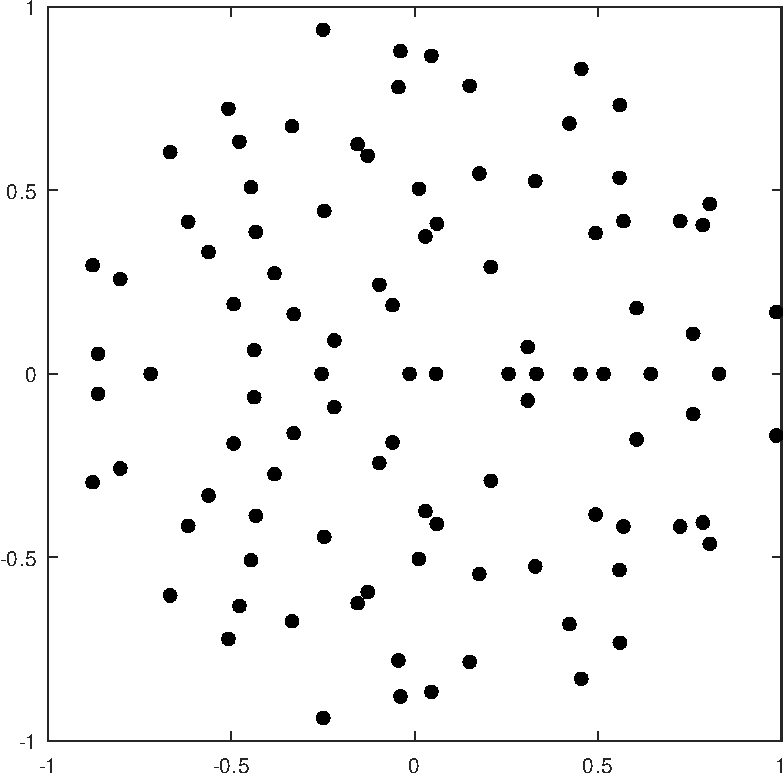
\includegraphics[scale=0.4]{fig/spectrum}} \hfill
    (b) \raisebox{-55mm}{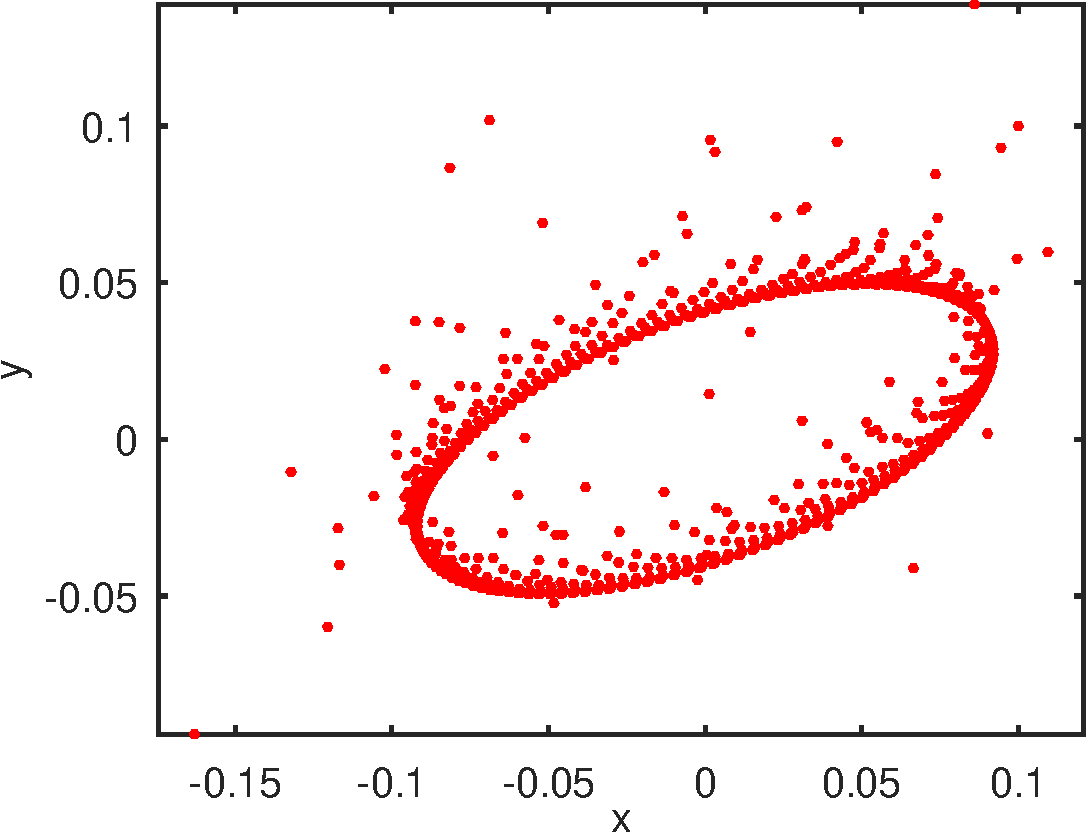
\includegraphics[scale=0.4]{fig/ellipse}} \\[5mm]
    (c) \raisebox{-55mm}{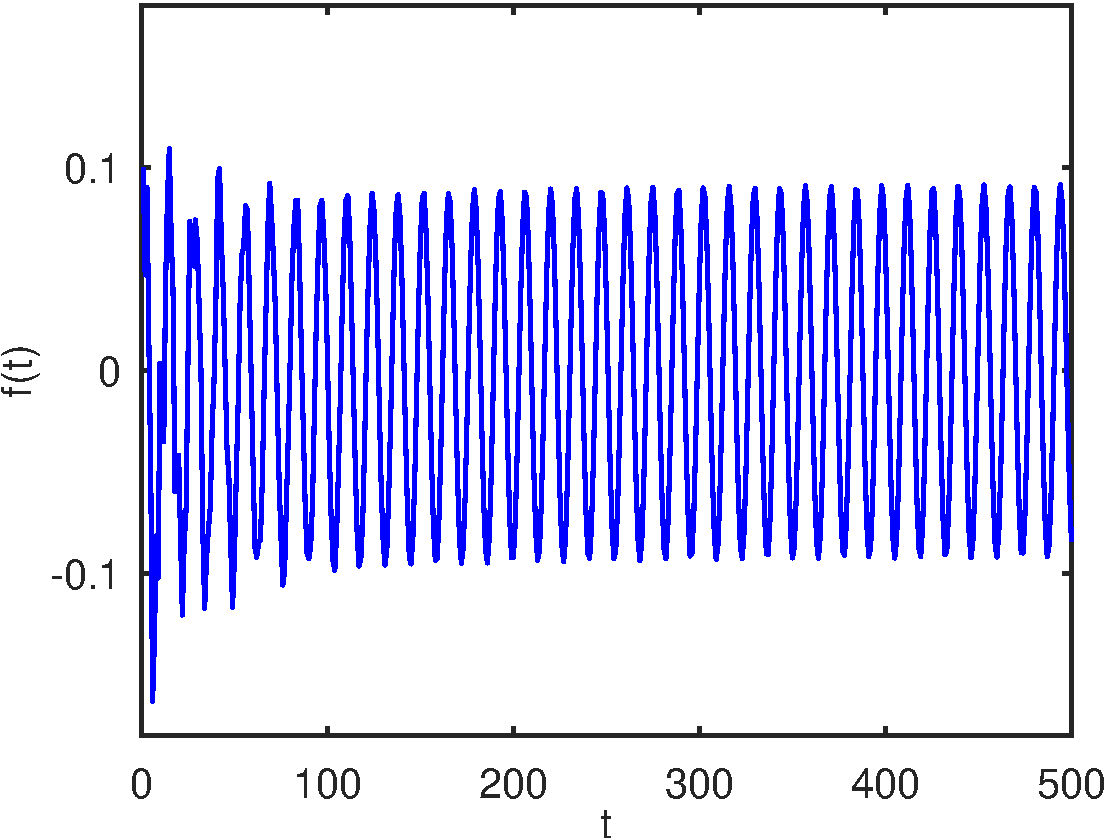
\includegraphics[scale=0.4]{fig/wave}}
  \caption{Dynamic system behavior of a pure random reservoir with unit spectral
	radius, with $N^\mathrm{res} = 100$ neurons:
    (a)~Eigenvalue spectrum of the reservoir matrix $W^\mathrm{res}$ with
	complex conjugate eigenvalue pairs in the complex plane.
    (b)~Visualization of $f(t)$ by planar projection. In the long run, we get an
	ellipse trajectory, thus only two dimensions (cf. \cref{twodim}).
    (c)~Projected to one (arbitrary) dimension, we have pure sinusoids with one
	single angular frequency for large $t$, sampled in large steps.}
  \label{ell}
\end{figure}

\begin{figure}
 \centering
 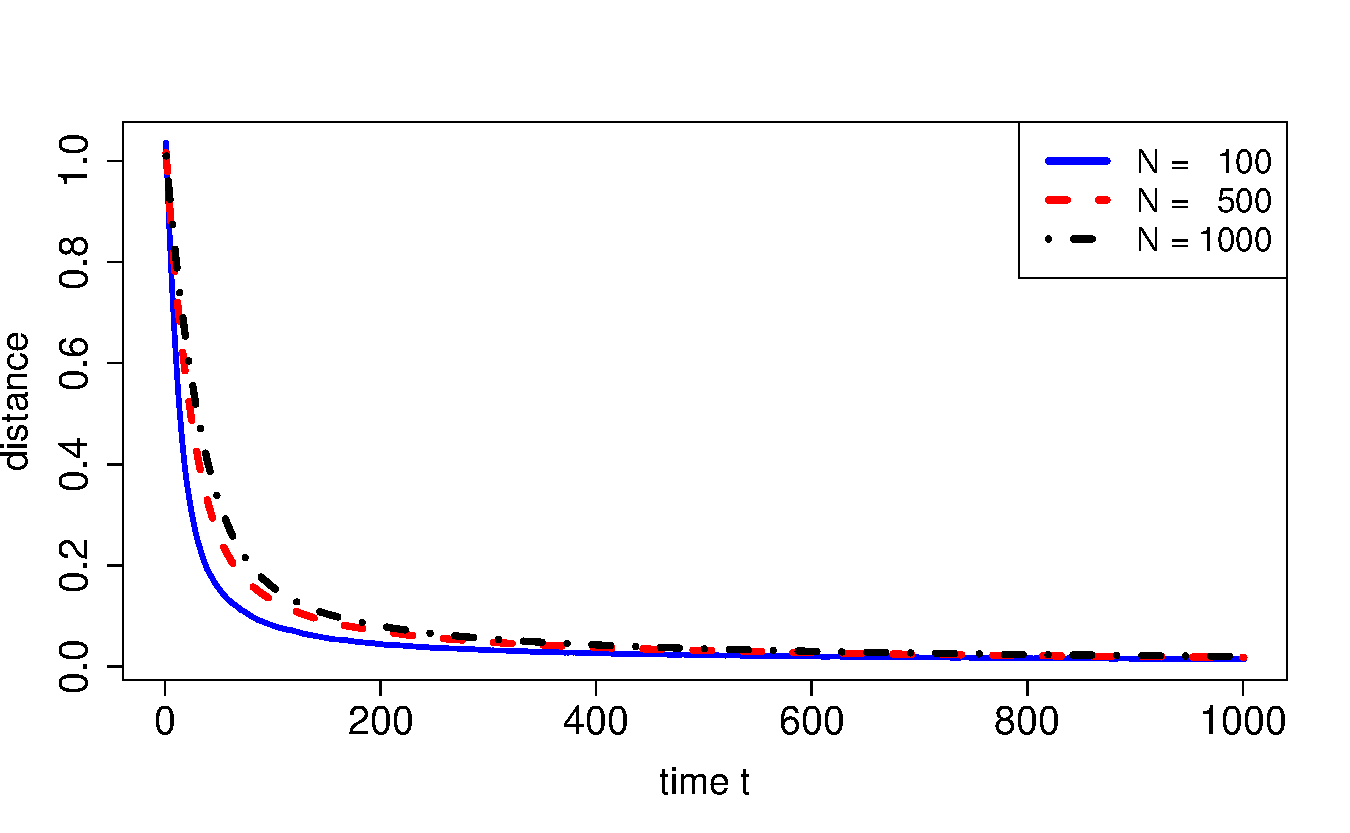
\includegraphics[width=0.7\textwidth]{fig/asymptot0} % asymptot1 for solid lines, 0 for dashed
  \caption{Asymptotic behavior of pure random reservoirs with unit spectral radius:
	The (Euclidean) distance between the actual value $f(t)$
	(according to \cref{form}) and its approximation by the final ellipse
	trajectory (\cref{twodim}) is almost zero already after a few hundred
	steps. The figure shows the distances for $N^\mathrm{res}=100$ (solid/blue), $N^\mathrm{res}=500$
	(dashed/red), and $N^\mathrm{res}=1000$ (dotted/black) random reservoir neurons,
	starting with a random vector of unit length, averaged over 1000 trials.}
  \label{asymptot}
\end{figure}

The long-term behavior of LRNNs is related to that of ESNs. For the latter,
usually the activation function is $\tanh$ and the spectral radius is smaller
than $1$. Then reservoirs with zero input collapse because of $|\!\tanh(z)| \le
|z|$ for all $z \in \mathbb{R}$ but the convergence may be rather slow,
nonetheless it guarantees contractivity and hence for any fixed input (not just
the origin) the system converges to a unique fixed point. This leads
to the so-called \emph{echo state property} \citep{MJ13}: Any random initial
state of a reservoir is forgotten such that, after a washout period, the current
network state is a function of the driving input. In contrast to ESNs, LRNNs
have linear activation and a spectral radius of exactly~$1$ (cf. \cref{thedef}).
But as we have just shown, there is a similar effect in the long run: The
network activity reduces to at most two dimensions which are independent from
the initial state of the network.

\section{Learning LRNNs}\label{learn}

Functions can be learned and approximated by LRNNs in two steps: First, as for
ESNs \citep{JH04}, we only learn the output weights $W^\mathrm{out}$ (cf.
\cref{output}); all other connections remain unchanged. The input weights
$W^\mathrm{in}$ and reservoir weights $W^\mathrm{res}$ are arbitrary random
values that are not changed (cf. \cref{thedef}). Nevertheless, in order to
obtain better numerical stability during the computation, they are adjusted as
follows:
\begin{itemize}
  \item Because of the linear activation, the spectral radius of the reservoir
	weights matrix $W^\mathrm{res}$ is set to $1$ (cf. \cref{thedef}).
	Otherwise, with increasing $t$, the values of $f(t) = W^t \cdot s$
	explode if the spectral radius is greater or vanish if the spectral
	radius is smaller than $1$ (cf. \cref{ellipse}). In consequence, the
	overall learning procedure behaves rather stable.
  \item The norms of the vectors in $W^\mathrm{in}$ and $W^\mathrm{res}$ should
	be balanced \citep{KLB12}. To achieve this, we initialize the reservoir
	neurons such that the reservoir start vector $r$ (with $N^\mathrm{res}$
	components) has unit norm by
	setting:
	\[ r = \frac{1}{\sqrt{N^\mathrm{res}}} \cdot \big[ 1 \cdots 1 \big]^\top \]
	It is part of the start vector $s = \left[ \begin{array}{c} S(0) \\ r
	\end{array} \right]$ (cf. \cref{define}).
  \item We usually employ fully connected graphs, i.e., all, especially the
	reservoir neurons are connected with each other because the
	connectivity has nearly no influence on the best reachable performance
	\citep{KLB12}.
\end{itemize}
Second, if possible, we reduce the network size (cf. \cref{reduce});
this often leads to better generalization and avoids overfitting. Thus, in
contrast to many other approaches, the network architecture is changed during
the learning process. In contrast to other approaches, we do not do this by
incremental derivation from the original network but in only one step.

\subsection{Learning the Output Weights}\label{output}

To learn the output weights $W^\mathrm{out}$, we run the input values from the
time series $S(0),\dots,S(n)$ through the network (in input receiving mode),
particularly through the reservoir. This means, we build the sequence of
corresponding reservoir states $R(0),\dots,R(n)$ where the reservoir start
vector $r$ in principle can be chosen arbitrarily but with all non-zero
entries (cf. \cref{chad}):
\begin{equation}\label{Res}
	R(t_0) = r \text{~and~} R(t+\tau) =
	\left[ W^\mathrm{in} ~~ W^\mathrm{res} \right] \cdot
	\left[ \begin{array}{c} S(t) \\ R(t) \end{array} \right]
\end{equation}
We want to predict the next input value $S(t+\tau)$, given the current input and
reservoir states $S(t)$ and $R(t)$. To achieve this, we comprise
all but the last input and reservoir states in one matrix $X$ with:
\begin{equation}\label{Xin}
    X = \left[ \begin{array}{ccc}
	S(0) & \cdots & S(n-1)\\
	R(0) & \cdots & R(n-1)
	\end{array} \right]
\end{equation}
Each output value shall correspond to the respective next input value $S(t+\tau)$.
Therefore, we compose another matrix
\begin{equation}\label{Yout}
	Y^\mathrm{out} = \big[ S(1)\ \cdots\ S(n) \big]
\end{equation}
consisting of the next values of the time series $S$ to be predicted
where the first value $S(0)$ clearly has to be omitted because it cannot be
predicted. We compute $Y^\mathrm{out}(t) = S(t+\tau)$ from $X(t)$ by assuming a
linear dependency:
\begin{equation}\label{linear}
	Y^\mathrm{out} = W^\mathrm{out} \cdot X
\end{equation}
Its solution can easily be determined as $W^\mathrm{out} = Y^\mathrm{out}/X$,
where $/$ denotes right matrix division, i.e., the operation of solving a linear
equation system, possibly applying the least squares method in case of an
overdetermined system, as implemented in many scientific programming languages
like Matlab \citep{HH17} or Octave \citep{EB+17}. Prediction of further values
is now possible (in output generating mode) as follows:
\begin{equation}\label{predict}
	\left[ \begin{array}{c} S(t+\tau) \\ R(t+\tau) \end{array} \right]
	= W \cdot \left[ \begin{array}{c} S(t) \\ R(t) \end{array} \right]
	\text{~with~} W \text{~as in \cref{matrix}}
\end{equation}

\begin{prop}[treatment of multiple sequences]\label{multi}
It is also possible to learn from multiple sequences at once. For this, let
several time series $S_1,\dots,S_K$ in $d$ dimensions with (not necessarily
identical) lengths $n_1,\dots,n_K$ be given. For each $S_k$ with $1 \le k \le
K$, we determine:
\begin{itemize}
  \item the sequence of corresponding reservoir states $R_k$ (according to
	\cref{Res}), taking always the same reservoir start vector $r$,
  \item the corresponding input matrix $X_k$ (according to \cref{Xin}), and
  \item the corresponding predicted output matrix $Y^\mathrm{out}_k$ (according to \cref{Yout}).
\end{itemize}
We aggregate the input and output matrices to $X = \big[ X_1 \cdots X_K \big]$
and $Y^\mathrm{out} = \big[ Y^\mathrm{out}_1 \cdots Y^\mathrm{out}_K \big]$ with
$n_1+\,\cdots\,+n_K$ columns each. Solving the linear matrix equation
$Y^\mathrm{out} = W^\mathrm{out} \cdot X$ (identical with \cref{linear})
finally yields the output weight matrix $W^\mathrm{out}$.
\end{prop}

This first phase of the learning procedure is related to a linear
\emph{autoregressive model} \citep{Aka69}. However, one important
difference to an autoregressive model is that for LRNNs the output does not only
depend on its own previous values and possibly white noise but on the complete
state of the possibly big reservoir whose dynamics is explicitly dealt with in
the reservoir matrix $W^\mathrm{res}$. The reservoir effectively allows us to do
arbitrary auxiliary computation such that any (non-linear) function $f(t)$ can
be approximated by an LRNN (cf.~\cref{approx}).

\subsection{An Approximation Theorem}

\begin{prop}\label{approx}
From a function $f(t)$ in $d \ge 1$ dimensions, let a
series of function values $f(t_0),\dots,f(t_n)$ be given. Then there is an
LRNN with the following properties:
\begin{enumerate}
  \item It runs exactly through all given $n+1$ function values, i.e., it approximates $f(t)$.
  \item It can effectively be learned by the LRNN learning procedure (\cref{output}).
\end{enumerate}
\end{prop}

\begin{proof}
First, we take the series of function values $f(t_0),\dots,f(t_n)$ and identify
them with the time series $S(0),\dots,S(n)$. After applying the LRNN learning
procedure, the LRNN runs through all given values, because by construction the
upper part $\big[ S(0) \cdots S(n-1) \big]$ of the matrix $X$ (cf. \cref{Xin})
and the matrix $Y^\mathrm{out}$ (cf. \cref{Yout}) consist of the series of
function values of $f$, provided that the linear
matrix equation $Y^\mathrm{out} = W^\mathrm{out} \cdot X$ (\cref{linear}) has at
least one solution.

Since \cref{linear} is equivalent to simultaneously solving the equations $y_k =
w_k \cdot X$, for $1 \le k \le N$ where $y_1,\dots,y_N$ and $w_1,\dots,w_N$
denote the row vectors of the matrices $Y^\mathrm{out}$ and $W^\mathrm{out}$,
respectively, the latter is the case if the rank of the coefficient matrix $X$
is equal to the rank of the augmented matrix $M_k = \big[ X ~~ y_k \big]^\top$
for every $k$. This leads to the equation $\mathrm{rank}(X) =
\min(N^\mathrm{in\,out}+N^\mathrm{res},n) = \mathrm{rank}(M_k) =
\min(N^\mathrm{in\,out}+N^\mathrm{res}+1,n)$. From this, it follows that
\begin{equation}\label{ineq}
	N^\mathrm{res} \ge n-N^\mathrm{in\,out}
\end{equation}
reservoir neurons have to be employed to guarantee at least one solution for the
$w_k$, provided that the rank of the matrix $X$ is maximal. For the latter, we
consider two cases:
\begin{itemize}
  \item If the rank of the upper part of the matrix $X$ (see above) is not
	maximal, then this does not cause any problems. We only have to replace
	$N^\mathrm{in\,out}$ by the actual rank of the upper part of the matrix
	$X$ in \cref{ineq}.
  \item The rank of the lower part $\big[ R(0) \cdots R(n-1) \big]$ of the
	matrix $X$ almost always has maximal rank, because we employ a random
	reservoir (cf. \cref{thedef}). Thus, a suitable reservoir does the job,
	which completes the proof.
	\vspace*{-5ex} %\qedhere
\end{itemize}
\end{proof}

Therefore, at least in theory, any time-dependent function $f(t)$ can be
interpolated, i.e., exactly approximated on the given function values and
continued on input other than nonnegative integer numbers (cf. \cref{general}),
although clearly not every function can be implemented by LRNNs, in particular
functions increasing faster than single-exponential (cf. \cref{exponential})
like $2^{2^t}$ (double-exponential) or $t\/!$ (factorial function). Also in
practice, the LRNN learning procedure performs rather well (cf. \cref{result}).
Nevertheless, the matrix $X$ may be ill-conditioned for long input sequences, because the reservoir state
sequence as part of the matrix $X$ reduces to at most two dimensions for large
$t$, independent of the number of reservoir neurons (cf. \cref{ellipse}). Hence,
the rank of the matrix $X$ may not be maximal and consequently \cref{linear} may not
be solvable numerically in practice (although we may have an equation system with
the same number of equations and unknowns). A simple increase of the number of
reservoir neurons does not help much.

However, one could learn not only the output weights $W^\mathrm{out}$ as in ESNs
but the complete transition matrix $W$: For this, we employ a random reservoir
state sequence matrix $\big[R(0) \cdots R(n) \big]$ with $N^\mathrm{res}$
reservoir neurons, considered as additional input. If all elements of this
matrix are random numbers, independently and identically distributed from the
standard normal distribution, its rank is almost always maximal. We then just
have to solve the linear matrix equation $Y = W \cdot X$ (cf. \cref{linear})
with
\[ Y = \left[ \begin{array}{ccc}
	S(1) & \cdots & S(n)\\
	R(1) & \cdots & R(n)
\end{array} \right] \]
and $X$ as in \cref{Xin}. By this, the input and reservoir weights
$W^\mathrm{in}$ and $W^\mathrm{res}$ are learned, not only the output weights
$W^\mathrm{out}$. But our experiments indicate that this procedure is less
reliable than the one with given, i.e., predefined random input and reservoir
weights and unit spectral radius for the reservoir (cf. \cref{output}).

The topic of learning all weights in the matrix $W$ is investigated
by \citet{PDW13} for ESNs with nonlinear activation function in the reservoir.
However, for LRNNs, the given input and reservoir weights $W^\mathrm{in}$ and
$W^\mathrm{res}$ together with the learned output weights $W^\mathrm{out}$
already provide the best approximation of the function $f(t)$. There is no need
to learn the input and reservoir weights, simply because LRNNs are completely
linearly activated RNNs (including the reservoir). If one tries to learn
$W^\mathrm{in}$ and $W^\mathrm{res}$ taking not only the output time series $S$
but additionally the reservoir state time series $R$ into account, then exactly
the given input and reservoir weights are learned if \cref{ineq} holds. Only
with nonlinear activation there is a learning effect.

\begin{remk}
\cref{approx} is related to the \emph{universal approximation theorem} for
feedforward neural networks \citep{Hor91}. It states that a (non-recurrent)
network with a linear output layer and at least one hidden layer activated by a
nonlinear, sigmoidal function can approximate any continuous function on a
closed and bounded subset of the $\mathbb{R}^n$ from one finite-dimensional
space to another with any desired non-zero amount of error, provided that the
network is given enough hidden neurons \citep[Sect.~6.4.1]{GBC16}. Since RNNs
are more general than feedforward networks, the universal approximation theorem
also holds for them \citep{MNM02}. Any measurable function can be
approximated with a (general) recurrent network arbitrarily well in probability
\citep{Ham00}.

Because of the completely linear activation, LRNNs cannot compute a nonlinear
function $f(x)$ from the (possibly multi-dimensional) input $x$. Nevertheless,
they can approximate any (possibly nonlinear) function over time $f(t)$, as
\cref{approx} shows. Another important difference between LRNNs and
nonlinearly activated feedforward neural networks is that LRNNs can learn
the function $f(t)$ efficiently. No gradient-descent method like backpropagation is
required; we just have to solve a linear equation system. Hence learning is as
easy as learning a single-layer perceptron, which however is restricted in
expressibility because only linearly separable functions can be represented.
\end{remk}

\begin{remk}
Any time series $S(0),\dots,S(n)$ can be generated by employing a backward shift
matrix, i.e., a binary matrix with $1$s on the subdiagonal and $0$s elsewhere
\citep[Sect.~0.9.7]{HJ13}, as transition matrix $W$ and $s = \big[ S(0) \cdots
S(n) \big]^\top$ as start vector. But such a network clearly would have no
ability to generalize to future data. Fortunately, this does not hold for a
transition matrix $W$ learned by the procedure in \cref{output}. Furthermore,
the eigenvalue spectrum of the backward shift matrix is empty, whereas that of
the learned $W$ is not, which is important for network size reduction
introduced in \cref{reduce}.
\end{remk}

\subsection{Network Size Reduction}\label{reduce}

To approximate a function exactly for sure, we need a large number
$N^\mathrm{res}$ of reservoir neurons in \cref{approx}. It is certainly a
good idea to lower this number. One could do this by simply taking a smaller
number of reservoir neurons, but then a good approximation cannot be guaranteed.
In what follows, we therefore reduce the dimensionality of the transition matrix $W$ in a
more controlled way -- after learning the output weights. Our procedure of
dimensionality reduction leads to smaller networks with sparse connectivity. In
contrast to other approaches, we do not learn the new network architecture by
incremental derivation from the original network, e.g., by removing unimportant
neurons or weights, but in only one step by inspecting the eigenvalues of the
transition matrix.

For ESNs, dimensionality reduction is considered, too, namely by means of
so-called \emph{conceptors} \citep{Jae14,Jae17,KOS21b}. These are special matrices which
restrict the reservoir dynamics to a linear subspace that is characteristic for
a specific pattern. However, as in principal component analysis (PCA) \citep{Jol11}, conceptors
reduce only the spatial dimensionality of the point cloud of the given data. In
contrast to this, for LRNNs, we reduce the transition matrix $W$ and hence take
also into account the temporal order of the data points in the time series. By
applying insights from linear algebra, the actual network size can be reduced
and not only the subspace of computation as with conceptors.

\begin{prop}
By \cref{chad}, the function $f(t) = W^t \cdot s$ can be rewritten by
means of the Jordan matrix of the transition matrix $W$ as $A \cdot J^t
\cdot y$, where the start vector can be chosen as non-zero constant, e.g., $y =
\big[ 1 \cdots 1 \big]^\top$. Furthermore, by \cref{jordan}, $f(t)$ can be
expressed as a sum of vectors $u = v \cdot J_m(\lambda)^t \cdot w$ where $w$ is
constant because it is part of the start vector~$y$. Then it follows from
\cref{infty} that for large $t$ the contribution of a Jordan component
vanishes if $\|v\| \approx 0$ and/or $|\lambda| \ll 1$.

In consequence, we can omit all Jordan components causing only small errors,
until a given threshold is exceeded. The error $E$ of a network can be estimated by the
root-mean-square error (RMSE) normalized to the number of all sample components
between input $x$ and predicted output $y$:
  \[ \mathrm{RMSE}(x,y) = \sqrt{\frac{1}{n} \sum_{t=1}^n \big\|x(t)-y(t)\big\|^2} \]
We shall omit all network components corresponding to Jordan blocks
$J_m(\lambda)$ with smallest errors as long as the
RMSE is below a given threshold $\theta$. Network components that are not
omitted are considered \emph{relevant}. Thus, from $A$, $J$, and
$y$ (according to \cref{chad}), we successively derive reduced matrices
$A$ and $J$ and the vector $y$ as follows:
\begin{itemize}
  \item Reduce $A$ to the rows corresponding to the input/output components and
	the columns corresponding to the relevant network components.
  \item Reduce $J$ to the rows and columns corresponding to the relevant
	network components.
  \item Reduce $y$ to the rows corresponding to the relevant network components.
\end{itemize}
\end{prop}

Note that the dimensionality reduction does not only lead to a smaller number of
reservoir neurons but also to a rather simple network structure: The transition
matrix $J$ (which comprises the reservoir weights $W^\mathrm{res}$ of
the reduced network) is a sparse matrix with non-zero elements only on the main
and immediately adjacent diagonals. Thus, the number of connections is in
$O(N)$, i.e., linear in the number of reservoir neurons, not quadratic -- as in
general.

\cref{proc} summarizes the overall learning procedure for LRNNs including
network size reduction. It has been implemented by the authors in Octave. Note
that, although the Jordan matrix $J$ (cf. \cref{jordan}) may
contain eigenvalues with multiplicity greater than $1$, Octave does not always
calculate exactly identical eigenvalues in this case. Therefore, we cluster the
computed eigenvalues as follows: If the distance in the complex plane between
eigenvalues is below some given small threshold $\delta$, they are put into the
same cluster which eventually is identified with its centroid. Thus it is a kind
of single linkage clustering \citep{GR69}. The complete implementation of the
learning procedure together with some case studies (cf. \cref{result}) is
available under the following link:
\begin{center}
	\url{http://github.com/OliverObst/decorating/}
\end{center}

\begin{figure}
\newcommand{\commt}[1]{\%~#1\\}%
\begin{algorithmic}[1]\State
	\commt{$d$-dimensional function, given sampled, as time series, and start vector}
	$S = \big[ f(0) \cdots f(n) \big]$\\
	$s = \left[ \begin{array}{c} S(0) \\ r \end{array} \right]$ where
		$r = \frac{1}{\sqrt{N^\mathrm{res}}} \cdot
		\big[ \underbrace{1 \cdots 1}_{N^\mathrm{res} \text{~times}} \big]^\top$\newline
	\\
	\commt{random initialization of reservoir and input weights}
	$W^\mathrm{in} = \mathrm{randn}(N,d)$\\
	$W^\mathrm{res} = \mathrm{randn}(N^\mathrm{res},N^\mathrm{res})$
		normalized to unit spectral radius\newline
	\\
	\commt{learn output weights by linear regression}
	$X = \left[W^t \cdot s\right]_{t=0,\dots,n}$\\
	$Y^\mathrm{out} = \big[ S(1)\ \cdots\ S(n) \big]$\\
	$W^\mathrm{out} = Y^\mathrm{out}/X$\newline
	\\
	\commt{transition matrix and its decomposition}
	$W = \left[ \begin{array}{cc}
		\multicolumn{2}{c}{W^\mathrm{out}}\\
		W^\mathrm{in} & W^\mathrm{res}
	\end{array} \right]$\\
	$J = \mathrm{jordan\_matrix}(W)$ with components sorted in decreasing order\\
	\quad with respect to $\mathrm{Error}(J_{\langle 1,\dots,k-1,k+1,\dots,K \rangle})$\\
	\quad where $K = \#$\,Jordan components in $J$\newline
	\\
	\commt{network size reduction (with binary search)}
	$L = 1$\\
	$R = K$\\
	while ($L \neq R$)\\
	\quad $M = \left\lfloor\frac{L+R}{2}\right\rfloor$\\
	\quad if $\mathrm{Error}(J_{\langle 1,\dots,M \rangle}) < \theta$\\
	\qquad then $R = M$\\
	\qquad else $L = M+1$\\
	return\big($M$\big)\newline
	\\
	\commt{subroutine $\mathrm{Error}(J_I)$}
	\commt{\quad compute error for Jordan matrix reduced to indexed components}
	\quad reduce $J$ to components indexed by $I$\\
	\quad $y = \big[ 1 \cdots 1 \big]^\top$\\
	\quad $Y = \left[J^t \cdot y\right]_{t=0,\dots,n}$\\
	\quad $A = X/Y$ with rows restricted to input/output dimensions\\
	return\big($\mathrm{RMSE}(S,A \cdot Y)$\big)
\end{algorithmic}
\caption{Pseudocode for learning LRNNs including network size reduction. A
binary search algorithm is employed for determining the relevant network
components with smallest errors. For this, the network components are sorted by
their RMSE. The program returns the number $M$ of relevant components in the
Jordan matrix $J$ (line 24). The subroutine $\mathrm{Error}(J_I)$ (lines 25-31)
computes the error of the predicted output for the Jordan matrix reduced to the
components indexed by $I$.}
\label{proc}
\end{figure}

\begin{exmp}\label{continued}
Let us illustrate the LRNN learning procedure (\cref{proc}) with the Fibonacci
series (\cref{fibonacci}). We start with the first values of the Fibonacci
series $f(0),\dots,f(n)$ as input $S$ (lines 1-3) and generate a random
reservoir of size $N^\mathrm{res}$ (lines 4-6). After learning the output
weights $W^\mathrm{out}$ (lines 7-10) and decomposing the resulting transition
matrix $W$ (lines 11-15), the network size reduction procedure (lines 16-24)
often yields minimal networks with only two reservoir neurons representing
\[
    f(t) \overset{\text{\cref{chad}}}{=} A \cdot J^t \cdot y \text{~with~}
	A \approx \left[ \frac{1}{\sqrt{5}} ~~ -\!\frac{1}{\sqrt{5}} \right] \text{~and~}
	J \approx \left[ \begin{array}{cc}
		\lambda_1 & 0\\
		0 & \lambda_2
   	\end{array} \right] \text{~for~}
	y = \left[ \begin{array}{c}
	1\\
	1
   \end{array} \right]
\]
where the eigenvalues $\lambda_1$ and $\lambda_2$ are as in Binet's formula
(\cref{binet}). For instance, for $N^\mathrm{res}=n=30$ and precision threshold
$\theta=0.001$, we obtain minimal networks in 32\% of the cases from $100$
trials. They belong to the best networks with respect to their RSME. Thus,
by employing a standard validation procedure, the LRNN in \cref{examples}\,c
actually can be derived numerically by the LRNN learning procedure with network
size reduction.
\end{exmp}

Note that the spectral radius of the reservoir weights matrix $W^\mathrm{res}$
remains $1$ all the time (cf. \cref{thedef}). However, after learning the output
weights $W^\mathrm{out}$, the spectral radius of the overall transition matrix
$W$ (according to \cref{matrix}) of size $n+1$ and hence of the matrix $J$ may
be greater than $1$ if the function $f(t)$ to be modeled is exponentially
increasing. This obviously holds for the Fibonacci series ($\lambda_1>1$).

\subsection{Complexity and Generalization of the Procedure}

\begin{prop}\label{complexity}
In both learning steps, it is possible to employ any of the many available fast
and constructive algorithms for linear regression and eigendecomposition
\citep{DDH07}. Therefore, the time complexity is just $O(N^3)$ for both output
weights learning and network size reduction. In theory, if we assume that
the basic numerical operations like $+$~and~$\cdot$ can be done in constant
time, the asymptotic complexity is even a bit better. In practice, however, the
complexity depends on the bit length of numbers in floating point arithmetic,
of course, and may be worse hence. The size of the learned network is in $O(N)$
(cf. \cref{reduce}).
\end{prop}

Note that, in contrast, feedforward networks with three threshold neurons
already are NP-hard to train \citep{BR92}. This results from the fact
that the universal approximation theorem for feedforward networks differs from
\cref{approx} because the former holds for multi-dimensional functions and
not only time-dependent input. In this light, the computational complexity of
$O(N^3)$ for LRNNs does not look overly expensive. It dominates the
overall time complexity of the whole learning procedure because it is not
embedded in a time-consuming iterative learning procedure (like backpropagation)
as in other state-of-the-art methods.

\begin{remk}
We observe that most of the results presented in this paper still
hold if the transition matrix $W$ contains complex numbers. This means in
particular that also complex functions can be learned (from complex-valued time
series) and represented by LRNNs (\cref{approx}).
Nonetheless, the long-term behavior of networks with a random complex transition
matrix $W$ differs from the one described in \cref{ellipse} because then
there are no longer pairs of complex conjugate eigenvalues.
\end{remk}

\section{Experiments}\label{result}

In this section, we demonstrate evaluation results for learning and predicting
time series, approximating them by a function $f(t)$ represented by an LRNN,
for several tasks. We consider the following benchmarks: multiple superimposed
oscillators, number puzzles, robot soccer simulation, and predicting stock
prices. All experiments are performed with a program written by the authors in
Octave \citep{EB+17} (cf. \cref{reduce}). Let us start with an example that
illustrates the overall method.

\begin{exmp}\label{quest}
The graphs of the functions $f_1(t) = 4\,t\,(1-t)$ (parabola) and $f_2(t) =
\sin(\pi\,t)$ (sinusoid) look rather similar for $t \in [0,1]$ (cf.
\cref{parasin}). Can both functions be learned and distinguished from each other
by our LRNN learning procedure (cf. \cref{learn})?
\end{exmp}

\begin{figure}
	\centering
	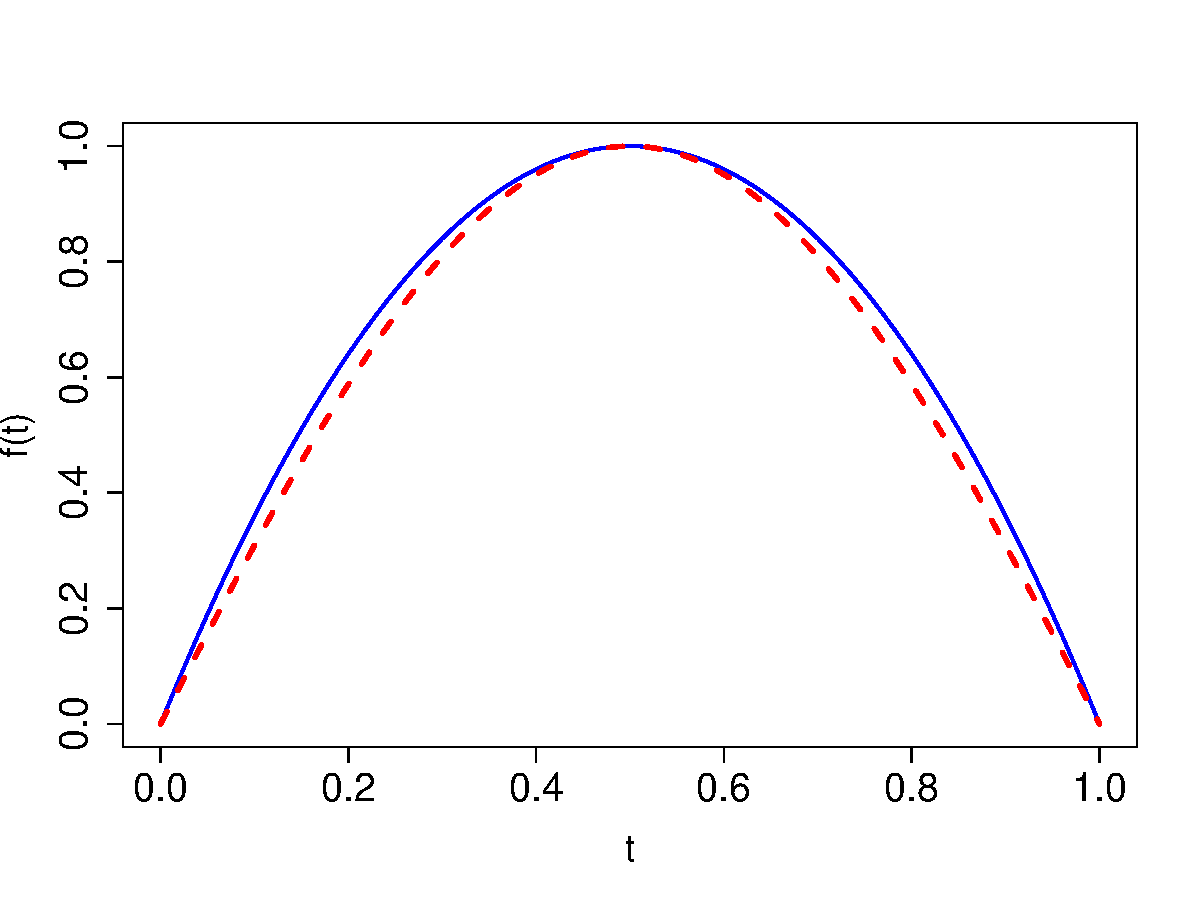
\includegraphics[width=0.55\textwidth]{fig/parasin2}
	\caption{Graphs for \cref{quest}: a parabola and a sinusoid.
	The question is: which one is which? Both can be learned and
	distinguished by LRNNs from the visually similar positive parts of the
	respective graphs, i.e., function values for $t \in [0, 1]$. In this
	interval, all values of the parabola (solid/blue) are greater than or equal
	to those of the sinusoid (dashed/red).}
	\label{parasin}
\end{figure}

To investigate this, we sample both graphs for $t \in [0,1]$ with time step
$\tau=0.01$. After that, we learn the output weights $W^\mathrm{out}$ (cf.
\cref{output}), starting with a large enough reservoir consisting of up to
$N^\mathrm{res} = 100$ neurons (cf. \cref{approx}). Finally, we reduce the
size of the overall transition matrix $W$ with precision threshold $\theta =
0.01$ and cluster threshold $\delta = 0.03$ (cf. \cref{reduce}). Minimal LRNNs
consist of $N_1 = 3$ neurons for
the parabola (cf. \cref{parabola}) and $N_2 = 2$ neurons for the sinusoid
(cf. \cref{ellipse}). The networks of minimal size are learned already with
$N^\mathrm{res} = 40$ reservoir neurons before network size reduction in about
77\% (parabola) or 99\% (sinusoid) of the trials (cf. \cref{dimens}).
Learning the parabola is more difficult because the corresponding transition
matrix $W$ (cf. \cref{parabola}) has no proper eigendecomposition according
to \cref{eigen} but only a Jordan decomposition according to \cref{jordan}.

\begin{figure}
	\centering
	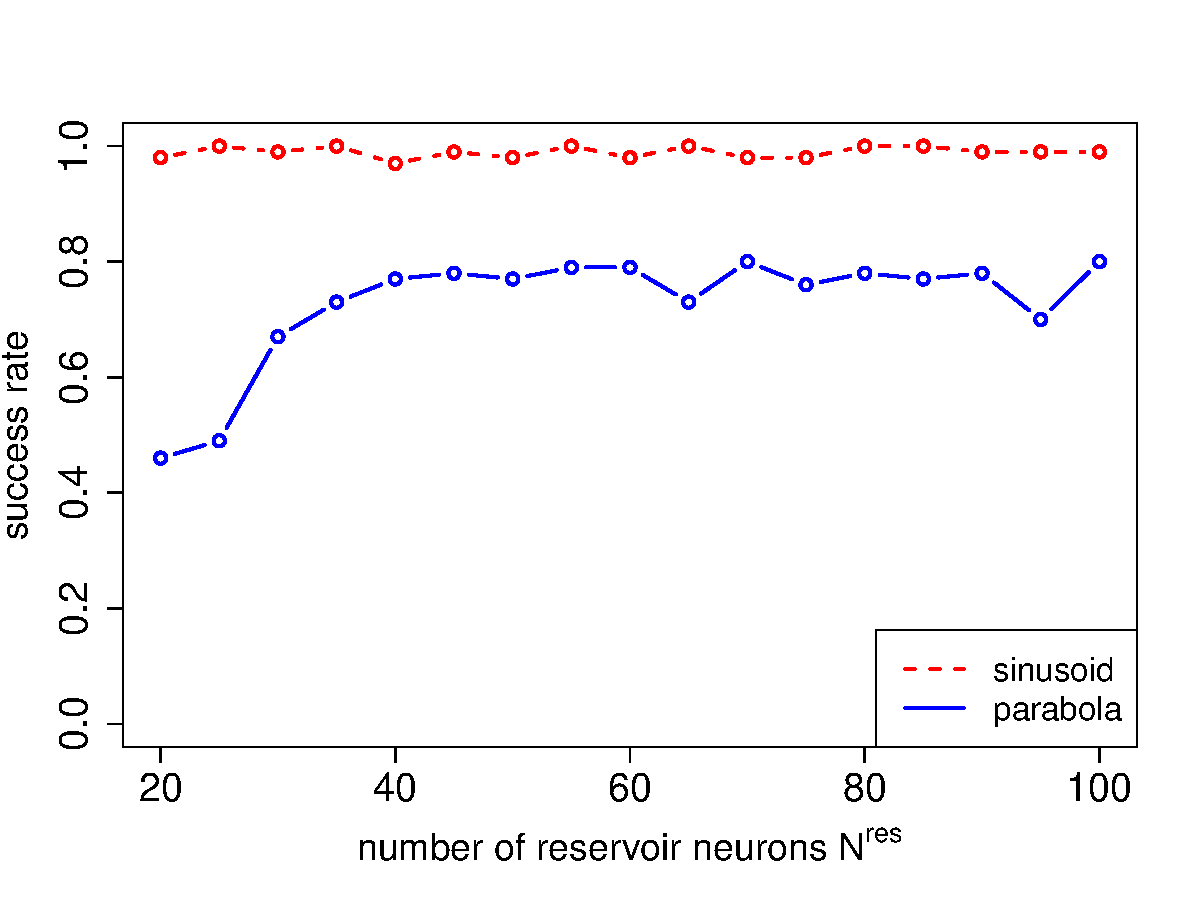
\includegraphics[width=0.55\textwidth]{fig/accuracy}
	\caption{For \cref{quest}, how often LRNNs of minimal size are
	learned after network size reduction, i.e., with $N_1 = 3$ neurons for
	the parabola and $N_2 = 2$ neurons for the sinusoid? The diagram shows
	the success rate of the learning procedure in this regard as a function
	of the number of reservoir neurons $N^\mathrm{res}$ before network size
	reduction (for 100 trials). Networks of minimal size are learned
	starting already with $N^\mathrm{res} = 40$ reservoir neurons in about
	77\% (parabola, solid/blue) or 99\% (sinusoid, dashed/red) of the
	trials.}
	\label{dimens}
\end{figure}

\subsection{Multiple Superimposed Oscillators}\label{mso}

\begin{exmp}\label{exmp}
Multiple superimposed oscillators (MSO) count as difficult benchmark problems
for RNNs \citep{KLB12,SW+07}. The corresponding time
series is generated by summing up several (pure) sinusoids. Formally
it is described by
	\[ S(t) = \sum\limits_{k=1}^K \sin(\alpha_k\,t) \]
where $K \le 8$ denotes the number of sinusoids and $\alpha_k \in \big\{ 0.200,
0.311, 0.420, 0.510, 0.630,\linebreak 0.740, 0.850, 0.970 \big\}$ their frequencies.
\end{exmp}

Various publications have investigated the MSO problem with different numbers of
sinusoids. We concentrate here solely on the most complex case $K=8$
because in contrast to other approaches it is still easy to learn for LRNNs.
Applying the LRNN learning procedure with precision threshold $\theta = 0.5$,
we arrive at LRNNs with only $N=16$ reservoir neurons and an RMSE less than
$10^{-5}$ (cf. \cref{signal}), if we start with a large enough reservoir (cf. \cref{mso8}). Since
two neurons are required for each frequency (cf. \cref{ellipse}), $2\,K=16$ is
the minimal size. Thus LRNNs outperform the previous state-of-the-art for the
MSO task with a minimal number of units. \citet{KLB12} report $N^\mathrm{res} =
68$ as the optimal reservoir size for ESNs, but in contrast to our approach,
this number is not further reduced.

\begin{figure}
  \centering
  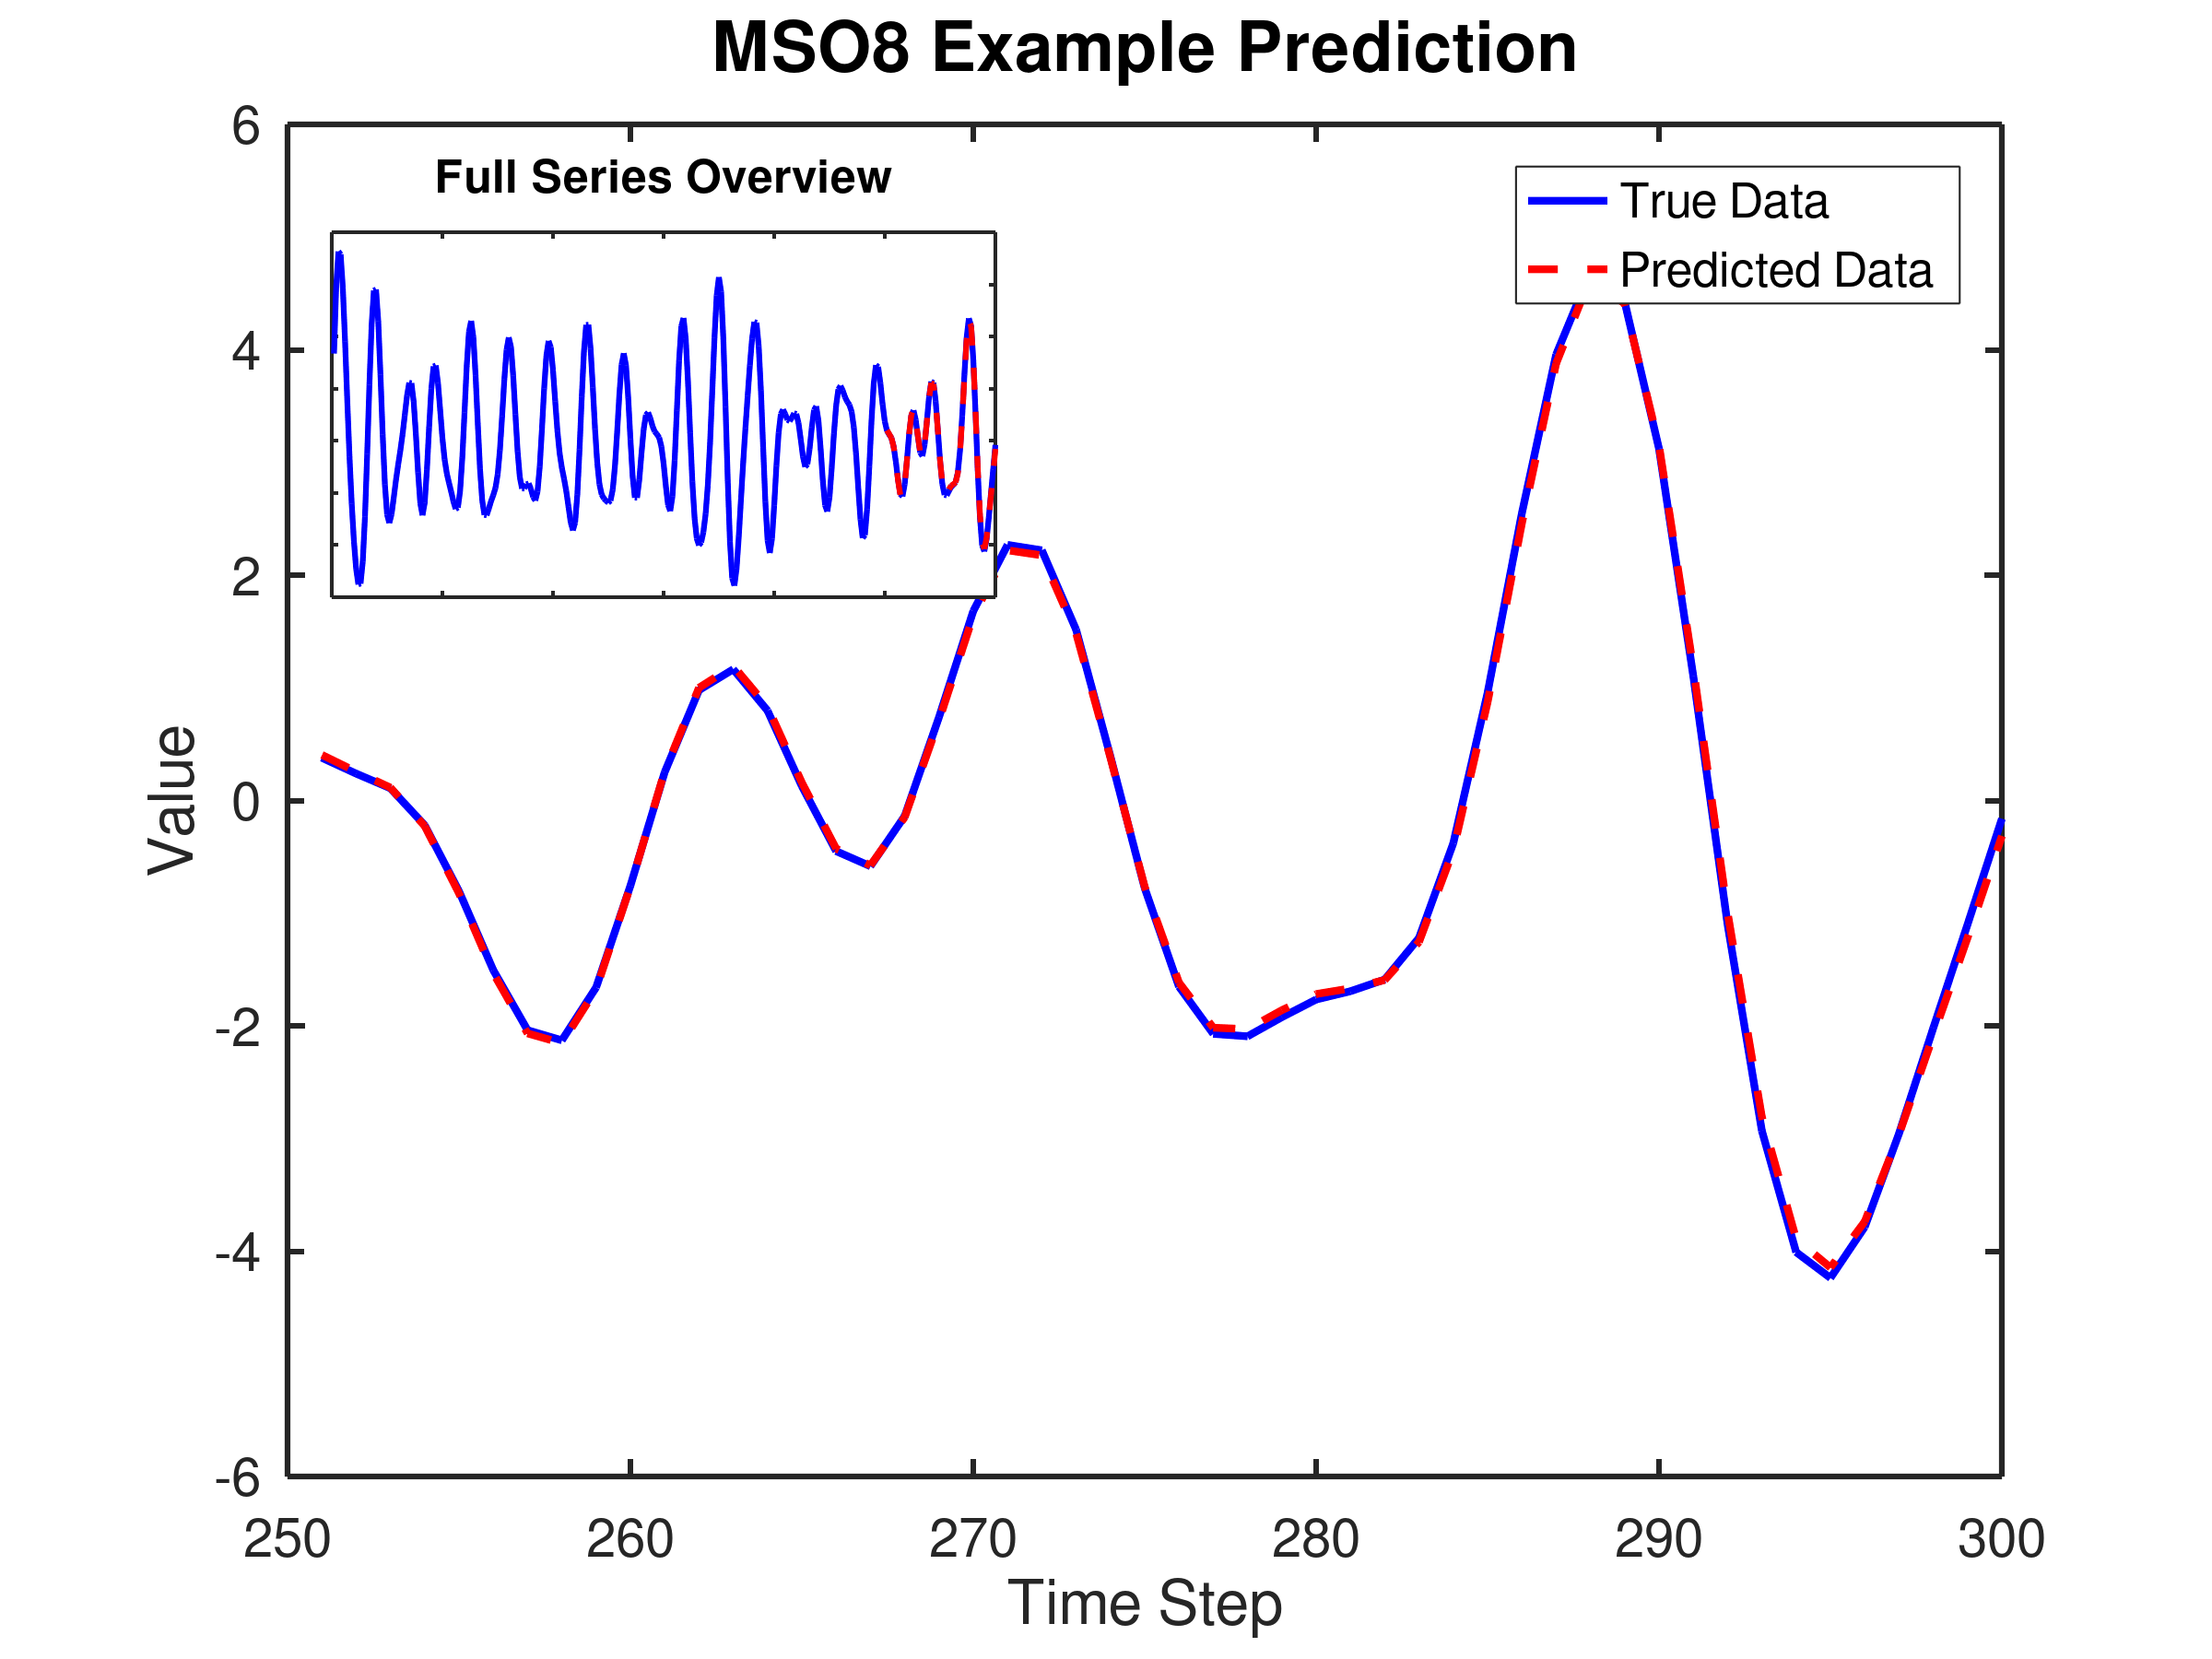
\includegraphics[width=0.65\textwidth]{fig/mso8_prediction_1}
  \caption{The signal $S(t)$ of $K=8$ multiple superimposed oscillators (for $1
	\le t \le 300$ and time step $\tau=1$) does not have a simple periodic
	structure (small figure). LRNN learning leads to minimal networks with
	only $N=16=2K$ reservoir neurons, i.e., two for each frequency in the
	signal, with RMSE less than $10^{-5}$ (dashed line). Other methods do
	not perform so well on the MSO benchmark (cf. dotted lines).}
  \label{signal}
\medskip
  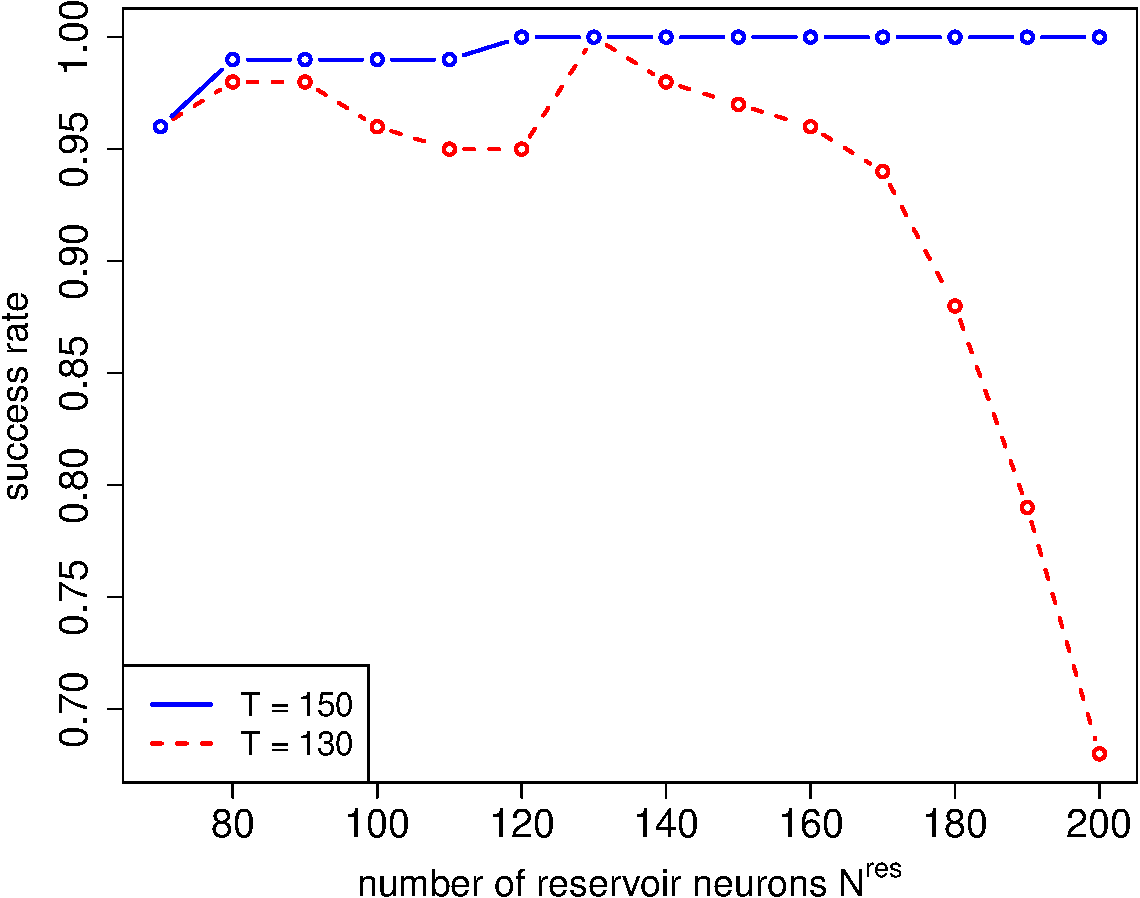
\includegraphics[width=0.56\textwidth]{fig/mso8}%
  \caption{Experimental results for the MSO benchmark ($K=8$). The diagram shows the
	success rate (from 100 trials): from an initial reservoir size of $N^\mathrm{res}$
	neurons, how often is the minimal LRNN with size
	$N=16$ learned? The two curves are for different lengths $T$ of the time series
	$S(t)$ used for training. Already for $T=150$ (solid/blue), a
	minimal-size LRNN is learned in at least 96\% of the trials if
	$N^\mathrm{res} \ge 70$. For these minimal LRNNs, the RMSE is smaller
	than $10^{-5}$. As one can see, for $T=130$ (dashed/red) the given
	information does not always suffice and leads to overfitting.}
  \label{mso8}
\end{figure}

For a more systematic evaluation, we generalize the MSO benchmark (\cref{exmp})
by considering $20$ times $K=8$ random frequencies $\alpha_1,\dots,\alpha_8$
uniformly distributed on the interval $[0,1]$. We take the first $250$ time
steps, i.e., $t=1,\dots,250$, as training data and the subsequent $50$ time
steps as testing data and compare the performance of LRNNs with other approaches
(cf. \cref{related}) with respect to their RSME on the testing data, partially
using the Python library Darts \citep[see also \url{http://unit8co.github.io/darts/}]{HLPN+22}  for
time series, including a simple baseline:

\begin{itemize}
  \item Baseline: Constantly predict the arithmetic mean of the training data.
  \item ARIMA: We use the AutoARIMA package from \citet{HK08}.
  \item ESN: For this, we adapt the simple sparse ESN demo by Mantas
	Luko\v{s}evi\v{c}ius from \url{http://mantas.info/code/simple_esn/}.
	We also used ReservoirPy~\citep{TPDH20}.
  \item LSTM: We employ the respective forecasting model implemented in Darts
	with hyperparameter optimization taking the last $50$ time steps of the
	training data for validation.
  \item LRNN: Here we adopt validation data as above and choose the best model
	with respect to the RMSE on the validation data from 100 trials.
\end{itemize}

\cref{sideways} shows the evaluation results. As one can see, LRNNs outperform
all other approaches on this benchmark by far. The reason for this is certainly
the network size reduction procedure (cf. \cref{reduce}), unique in our approach,
because it exactly selects the relevant components of the network: Each complex
conjugate
eigenvalue pair corresponds to one of the frequencies $\alpha_1,\dots,\alpha_8$.
In general, an LRNN with $2K$ neurons suffices to represent a signal, which
might be a musical harmony \citep{Sto17b}, consisting of $K$ sinusoids (cf.
\cref{ellipse}). It can be learned by the LRNN learning procedure with network
size reduction. However, if several frequencies are close to each other (cf.
example~\#1 in \cref{sideways}) or are rather small (cf. example~\#12), then
LRNNs do not perform quite so well.
	
\begin{sidewaystable}
  \centering\small
  \begin{tabular}{c*{8}{p{8mm}}cccc@{\,+\,}cccc}
     \toprule
	\# & \multicolumn{8}{l}{frequencies} & Baseline & ARIMA & ESN & \multicolumn{3}{c}{LSTM} & \multicolumn{2}{c}{LRNN}\\
	& $\alpha_1$ & $\alpha_2$ & $\alpha_3$ & $\alpha_4$ & $\alpha_5$ & $\alpha_6$ & $\alpha_7$ & $\alpha_8$ & RMSE & RMSE & RMSE & \multicolumn{2}{c}{units} & RMSE & $N$ & RMSE\\ \midrule
	1 & 0.334 & 0.336 & 0.399 & 0.403 & 0.412 & 0.438 & 0.442 & 0.724 & 2.05613 & 2.07496 & 0.23208 & 5 & 32 & 0.16038 & 10 & \textbf{0.04761}\\
	2 & 0.049 & 0.091 & 0.161 & 0.292 & 0.472 & 0.715 & 0.832 & 0.997 & 2.25490 & 3.06428 & 0.19716 & 10 & 2 & 0.19218 & 16 & \textbf{0.00051}\\
	3 & 0.308 & 0.521 & 0.597 & 0.607 & 0.736 & 0.766 & 0.924 & 0.957 & 1.34810 & 1.46533 & 0.13680 & 5 & 8 & 0.11722 & 16 & \textbf{0.00060}\\
	4 & 0.031 & 0.348 & 0.448 & 0.476 & 0.476 & 0.613 & 0.628 & 0.833 & 2.03748 & 2.13161 & 0.25979 & 5 & 8 & 0.19209 & 14 & \textbf{0.00003}\\
	5 & 0.059 & 0.239 & 0.324 & 0.421 & 0.437 & 0.519 & 0.747 & 0.777 & 1.68045 & 2.41015 & 0.16561 & 10 & 1 & 0.14548 & 16 & \textbf{0.00011}\\
	6 & 0.013 & 0.029 & 0.262 & 0.543 & 0.636 & 0.705 & 0.740 & 0.807 & 1.79038 & 2.91774 & 0.19343 & 5 & 4 & 0.16770 & 16 & \textbf{0.00038}\\
	7 & 0.155 & 0.226 & 0.286 & 0.512 & 0.661 & 0.692 & 0.746 & 0.930 & 1.48729 & 1.75658 & 0.13109 & 5 & 4 & 0.13761 & 16 & \textbf{0.00012}\\
	8 & 0.017 & 0.027 & 0.273 & 0.475 & 0.616 & 0.848 & 0.962 & 0.989 & 1.87712 & 2.66991 & 0.22200 & 5 & 2 & 0.16481 & 16 & \textbf{0.02033}\\
	9 & 0.092 & 0.318 & 0.335 & 0.413 & 0.593 & 0.743 & 0.747 & 0.799 & 1.84272 & 2.31084 & 0.22680 & 5 & 64 & 0.16025 & 16 & \textbf{0.00142}\\
	10 & 0.108 & 0.122 & 0.262 & 0.307 & 0.391 & 0.577 & 0.589 & 0.603 & 1.64237 & 1.66822 & 0.18361 & 10 & 16 & 0.13289 & 16 & \textbf{0.00772}\\
	11 & 0.071 & 0.264 & 0.557 & 0.609 & 0.641 & 0.719 & 0.853 & 0.964 & 1.71070 & 2.01792 & 0.13613 & 5 & 16 & 0.14964 & 16 & \textbf{0.00003}\\
	12 & 0.036 & 0.052 & 0.062 & 0.222 & 0.279 & 0.316 & 0.563 & 0.672 & 1.52224 & 1.83523 & 0.18562 & 10 & 8 & \textbf{0.15571} & 14 & 0.15984\\
	13 & 0.036 & 0.481 & 0.571 & 0.724 & 0.750 & 0.750 & 0.864 & 0.898 & 2.51888 & 2.50217 & 0.15961 & 5 & 16 & 0.22408 & 14 & \textbf{0.00067}\\
	14 & 0.175 & 0.220 & 0.258 & 0.419 & 0.487 & 0.513 & 0.628 & 0.663 & 2.17787 & 1.90370 & 0.23698 & 5 & 8 & 0.19731 & 16 & \textbf{0.00069}\\
	15 & 0.185 & 0.300 & 0.461 & 0.751 & 0.814 & 0.833 & 0.840 & 0.992 & 2.18527 & 1.63141 & 0.15527 & 5 & 2 & 0.20659 & 14 & \textbf{0.03709}\\
	16 & 0.088 & 0.120 & 0.137 & 0.245 & 0.478 & 0.793 & 0.797 & 0.992 & 2.27108 & 2.51581 & 0.15872 & 10 & 1 & 0.19325 & 16 & \textbf{0.01439}\\
	17 & 0.002 & 0.242 & 0.348 & 0.503 & 0.734 & 0.748 & 0.759 & 0.862 & 1.47542 & 1.76223 & 0.23496 & 10 & 8 & 0.13808 & 16 & \textbf{0.00150}\\
	18 & 0.018 & 0.352 & 0.583 & 0.625 & 0.714 & 0.824 & 0.838 & 0.888 & 2.44582 & 2.71492 & 0.24585 & 5 & 32 & 0.25433 & 16 & \textbf{0.00010}\\
	19 & 0.046 & 0.105 & 0.263 & 0.351 & 0.517 & 0.556 & 0.758 & 0.807 & 1.79806 & 2.24052 & 0.18220 & 5 & 16 & 0.18124 & 16 & \textbf{0.00005}\\
	20 & 0.091 & 0.141 & 0.375 & 0.578 & 0.686 & 0.785 & 0.951 & 0.996 & 2.05839 & 2.21768 & 0.15490 & 5 & 32 & 0.17551 & 16 & \textbf{0.00001}\\
	\bottomrule
  \end{tabular}
\caption{Evaluation results for 20 generalized MSO examples with 8 randomly
generated frequencies each. The best performing approach is highlighted by bold
face. For the LSTMs, the number of input and hidden units of the best performing
neural network is given. For LRNNs, the network size $N$ after network size
reduction is shown.}
\label{sideways}
\end{sidewaystable}

\subsection{Solving Number Puzzles}

\begin{exmp}
Number series tests are a popular type of intelligence test. The function
represented by a number series can often be learned also by artificial neural
networks, in particular RNNs. \citet{GW13} list 20 number puzzles \citep[cf.][]{RK11}.
Among them are the series:

\[ \begin{array}{c@{\,=\,}lc@{\,=\,}l}
	S_8 & [28,33,31,36,34,39,37,42] & f(t) & f(t-2) + 3\\[3pt]
	S_9 & [3,6,12,24,48,96,192,384] & f(t) & 2 f(t-1)\\[3pt]
	S_{15} & [6,9,18,21,42,45,90,93] & f(t) & 2 f(t-2) + 4.5 + 1.5 (-1)^{t-1}\\[3pt]
	S_{19} & [8,12,16,20,24,28,32,36] & f(t) & f(t-1) + 4
\end{array} \]
\end{exmp}

We apply the LRNN learning procedure to all 20 number puzzles taking small
reservoirs because the number series are short. As a side effect, this leads to
learning more general functions, which seems to be fully adequate because number
puzzles are usually presented to humans. The first 7 of 8 elements of each
series are given as input. In each trial, we repeatedly generate LRNNs, until the
RMSE is smaller than $\theta=0.1$. Then the last (8-th) element of the
respective series is predicted (according to \cref{predict}) and rounded to the
nearest integer because all considered number series are integer.

\cref{table} lists the percentages of correct predictions of the last
element for different settings. Here, the series with definitions recurring to
$f(t-2)$ but not $f(t-1)$, e.g., $S_8$ and $S_{15}$, turned out to be the most
difficult. If we now just add the previous values of the time series, i.e., $f(t-2)$,
as clue to the input, then the correctness of the procedure increases
significantly: For 19 of 20 number puzzles, the most frequently predicted last
element (simple majority) is the correct one. It is predicted in 76.5\% on
average over all trials and number puzzles. Let us remark that the whole
evaluation with altogether $20 \cdot 50 \cdot 1000 = 1\,000\,000$ trials
including possibly repeated network generation and network size reduction ran in
only a few minutes on standard hardware.

\begin{table}[t]
  \centering
  \sisetup{table-number-alignment = center, %
	table-figures-integer = 3, table-figures-decimal = 1, table-figures-exponent = 0, %
	table-space-text-post = \% }%
  \begin{tabular}{cSSSSS}
	\toprule
 	\head{series} & \head{$N^\mathrm{res}=3$}& \head{$N^\mathrm{res}=4$} & \head{$N^\mathrm{res}=5$} & \head{with reduction} & \head{plus clue}\\ \midrule
	$S_{1}$ & 2.2\% & 1.3\% & 1.3\% & 0.8\% & 33.4\% \\
	$S_{2}$ & 37.6\% & 42.2\% & 29.4\% & 32.0\% & 100.0\% \\
	$S_{3}$ & 5.4\% & 4.1\% & 1.1\% & 3.2\% & 100.0\% \\
	$S_{4}$ & 23.8\% & 24.2\% & 16.8\% & 23.2\% & 99.9\% \\
	$S_{5}$ & 56.9\% & 57.6\% & 44.2\% & 44.7\% & 99.7\% \\
	$S_{6}$ & 31.7\% & 33.7\% & 16.1\% & 11.0\% & 100.0\% \\
	$S_{7}$ & 72.8\% & 68.2\% & 56.2\% & 64.5\% & 100.0\% \\
	$S_{8}$ & 5.1\% & 3.4\% & 1.3\% & 1.8\% & 76.3\% \\
	$S_{9}$ & 100.0\% & 100.0\% & 100.0\% & 100.0\% & 100.0\% \\
	$S_{10}$ & 48.9\% & 71.5\% & 67.6\% & 72.6\% & 100.0\% \\
	$S_{11}$ & 10.6\% & 9.0\% & 3.4\% & 3.7\% & 100.0\% \\
	$S_{12}$ & 23.8\% & 21.1\% & 11.0\% & 8.5\% & 43.2\% \\
	$S_{13}$ & 56.5\% & 58.1\% & 41.5\% & 47.2\% & 99.8\% \\
	$S_{14}$ & 6.7\% & 7.4\% & 2.1\% & 2.7\% & 87.1\% \\
	$S_{15}$ & 1.6\% & 2.6\% & 2.5\% & 0.3\% & 1.1\% \\
	$S_{16}$ & 6.8\% & 5.9\% & 3.4\% & 2.9\% & 73.3\% \\
	$S_{17}$ & 11.9\% & 12.0\% & 6.8\% & 6.6\% & 41.0\% \\
	$S_{18}$ & 3.1\% & 2.0\% & 1.1\% & 0.9\% & 18.0\% \\
	$S_{19}$ & 59.6\% & 70.1\% & 72.0\% & 77.8\% & 99.8\% \\
	$S_{20}$ & 1.5\% & 0.5\% & 0.6\% & 0.5\% & 57.2\% \\ \bottomrule
  \end{tabular}
  \caption{Percentages of correct predictions of the last element for 20 number
	puzzles \citep{RK11,GW13} in 1000 trials for different settings:
	(a)~with fixed reservoir size $N^\mathrm{res}=3,4,5$; (b)~with network size
	reduction starting with $N^\mathrm{res}=7$ reservoir neurons; (c)~same
	procedure but in addition always the previous series value is used as clue.}
  \label{table}
\end{table}

\subsection{Replaying Soccer Games}\label{soccer}

RoboCup \citep{KA+97} is an international scientific robot competition in which
teams of multiple robots compete against each other. Its different leagues
provide many sources of robotics data that can be used for further analysis and
application of machine learning. A \emph{soccer simulation} game lasts 10\,mins and is
divided into 6000 time steps where the length of each cycle is 100\,ms. Logfiles
contain information about the game, in particular about the current positions of
all players and the ball including velocity and orientation for each cycle.
\citet{MO+19} describe a research dataset using some of the released binaries of
the RoboCup 2D soccer simulation league \citep{CDF+03,GFG16} from 2016 and 2017
\citep{MO+18}. In our experiments we evaluated ten games of the
top-five teams (available from \url{http://bitbucket.org/oliverobst/robocupsimdata}),
considering only the $(x,y)$-coordinates of the ball and the altogether 22
players for all time points during the so-called \enquote{play-on}
mode.

\begin{table}
\centering
\sisetup{table-number-alignment = center,  % group-digits = false,
	      table-figures-integer = 1, table-figures-decimal = 5, table-figures-exponent = 0}%
\begin{tabular}[b]{cSScc}
	\toprule
	\head{game} & \head{RMSE\,(1)} & \head{RMSE\,(2)} & \head{$N$} & \head{reduction}\\ \midrule
	\#1 & 0.00000 & 0.78581 & 385 & 29.5\%\\
	\#2 & 0.00001 & 0.96911 & 403 & 26.2\% \\
	\#3 & 0.00004 & 0.97680 & 390 & 28.6\% \\
	\#4 & 0.00000 & 0.97696 & 406 & 25.6\% \\
	\#5 & 0.00000 & 0.98425 & 437 & 20.0\% \\
	\#6 & 0.00000 & 0.47939 & 354 & 35.2\% \\
	\#7 & 0.00000 & 0.78731 & 390 & 28.6\% \\
	\#8 & 0.00255 & 0.98787 & 385 & 29.5\% \\
	\#9 & 0.00000 & 0.88518 & 342 & 37.4\% \\
	\#10 & 0.00000 & 0.96043 & 376 & 31.1\% \\
	\bottomrule
  \end{tabular}
  \caption{For ten RoboCup simulation games, an LRNN is learned with initially
	$N = 500+46 = 546$ neurons. The table shows the RMSE
	(1)~before and (2)~after dimensionality reduction where $\theta=1$\,m. The
	network size can be reduced significantly -- 29.2\% on average
	(last column).}
  \label{robocup}
\end{table}

For LRNN learning, we use only every $10^\text{th}$ time step of each 6000 step game with $d =
2+2 \cdot 22 = 46$ input dimensions and start with a reservoir consisting of
$N^\mathrm{res} = 500$ neurons. We repeat the learning procedure until the RMSE
is smaller than $1$; on average, already two attempts suffice for this. This
means, if we replay the game by the learned LRNN (in output generating mode)
then on average the predicted positions deviate less than 1\,m from the real
ones (Euclidean distance) -- over the whole length of the game (cf.
\cref{game}). Network size reduction leads to significantly less neurons
compared to the original number $N = 46+500 = 546$ -- on average 29.2\% if we
concentrate on the relevant components for the ball trajectory (cf.
\cref{robocup}). Note that the size of the learned network is in $O(N)$ (cf.
\cref{complexity}). Thus the LRNN model is definitely smaller than the
original time series representation of a game. The complete learning procedure
runs in less than a minute on standard hardware.

\begin{figure}[htb]
  \centering
  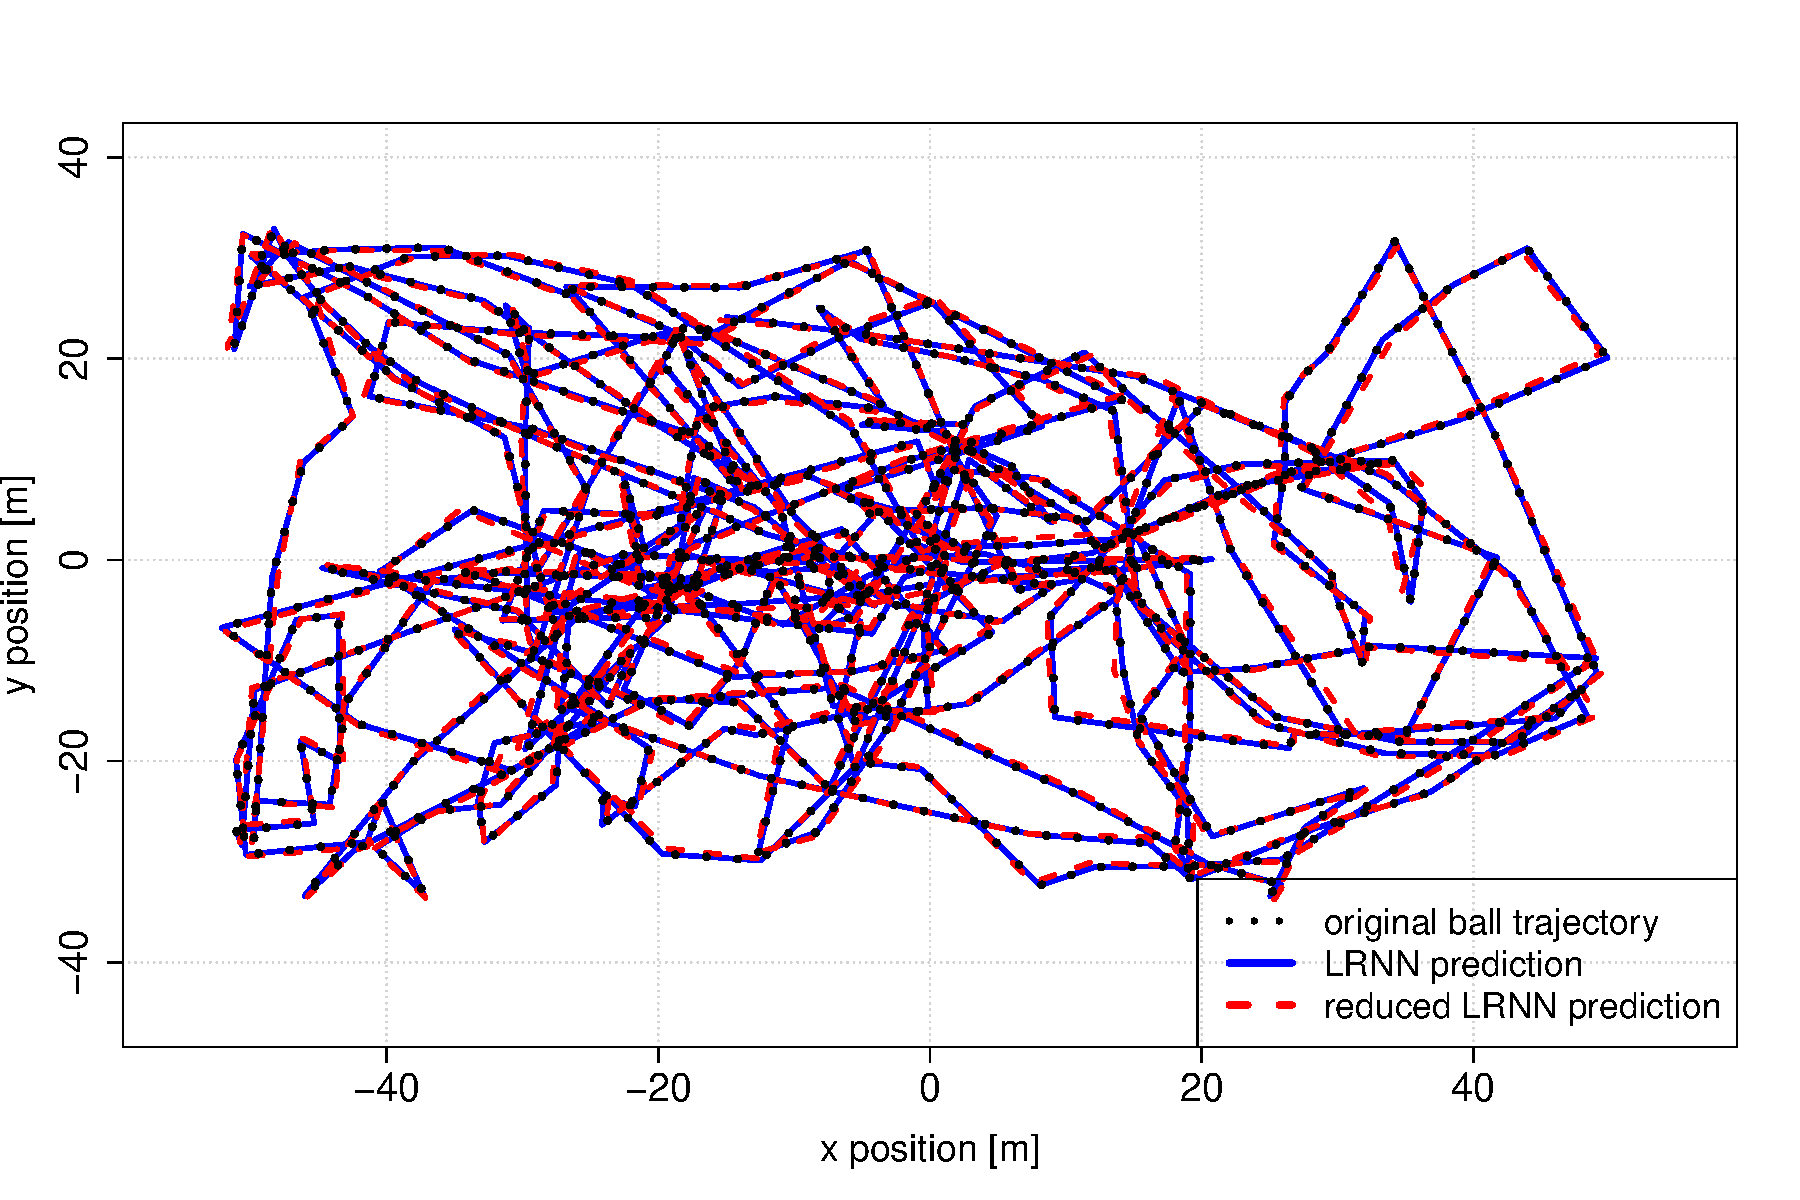
\includegraphics[width=0.8\columnwidth]{fig/game6}
  \caption{Ball trajectory of RoboCup 2D soccer simulation game \#6
	(\emph{Oxsy}~0 versus \emph{Gliders}~2016) on a pitch of size
	$105\,\mathrm{m} \times 68\,\mathrm{m}$. For all time steps, the
	original trajectory of the ball during play is shown (dotted/black). The
	game can be replayed by an LRNN with $N = 500+46 = 546$ neurons with high
	accuracy (solid/blue). The reduced network with $N = 354$ reservoir
	neurons still mimics the trajectory with only small error (dashed/red).
	\label{game}}
\end{figure}

\cref{multi} shows how we can learn from multiple time series at once. This is
also helpful here because by this procedure we can investigate the overall
behavior of a specific robot soccer agent. As example for this, we consider the
trajectories of the goalkeeper of the RoboCup simulation team FRA-UNIted during
the seeding and the qualifying round of RoboCup Japan Open 2020 (see
\url{http://bit.ly/japanopen2020ssim}). For learning one LRNN from this, we employ a
reservoir with $N^\mathrm{res} = 1000$ neurons, adopt again a maximum threshold
for the RMSE of $\theta = 1$\,m, and only use every $20^\text{th}$ step of each of the
$7$ games. The overall trajectory of the FRA-UNIted goalkeeper can be learned
easily then (cf. \cref{frankfurt}). From this, one may conclude that the
goalkeeper takes up three basic positions in front of the goal, does not
approach the centre line more than about 30\,m and hardly leaves the centre
line.

\begin{figure}
\centering
\hfill %
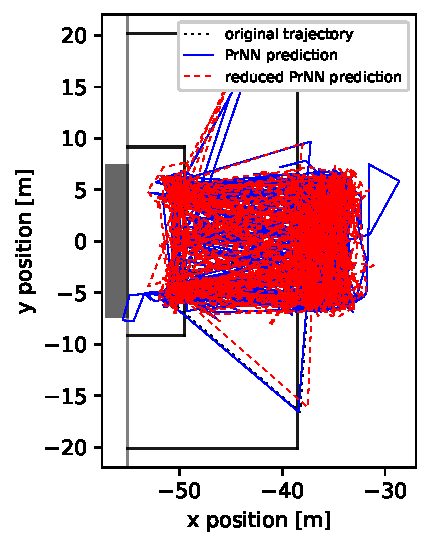
\includegraphics[width=0.34\columnwidth]{fig/goalie}     % 3450x4373
\hfill %
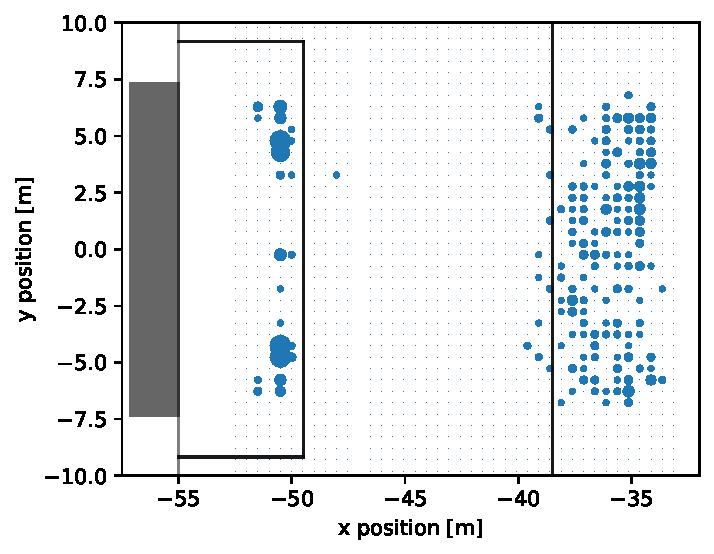
\includegraphics[width=0.57\columnwidth]{fig/goalievisits} % 5717x4437
\hfill %
\caption{Left: Trajectory of the FRA-UNIted goalkeeper in front of the goal
during games at the RoboCup Japan Open 2020. Right: Dots (in blue) mark positions
that were visited more than three times (larger dots: more visits, 0.5\,m resolution),
information that can be derived from predictions, highlighting three larger,
frequently visited regions in front of the goal.}
\label{frankfurt}
\end{figure}

\subsection{Predicting Stock Prices}\label{stock}

Stock price prediction is a topic that receives a considerable amount of
attention in finance. Complexity of markets resulting in multiple and sudden
changes in trends of stock prices make their prediction a challenge.
Consequently, a number of different approaches and methods have been developed.
\citet{Lit20} analyzes $30$ different stocks by ARIMA and LRNNs using the
closing stock prices 2016--2019. The stock price time series (consisting of
$762$ data points each) are split into training and testing data, with the first
80\% of each series for training and the final 20\% for evaluation. For a
representative comparison, the RMSE of the predictions on every stock in the set
is calculated. The average RMSE using LRNNs with $N^\mathrm{res}=600$ reservoir
neurons is $E_\mathrm{test}=18.40${\,\euro}, lower than the average RMSE using
ARIMA models with seasonal patterns modeled using Fourier terms
\citep[p.~321]{HA13} which is $E_\mathrm{test}=24.23${\,\euro}. For shorter term
predictions of 60 steps, it is possible to slightly reduce the RMSE further to
E$_\mathrm{test}=17.46${\,\euro} by using smaller LRNNs of $N^\mathrm{res}=200$
reservoir neurons and a smaller training set of $240$ data points. With an
average stock price of $286.71${\,\euro} of all stocks in the set, the average
deviation is only~6.1\%.

Apart from the good prediction results, LRNNs have the advantage that they allow
the prediction of multiple stocks at the same time. An LRNN can read in 30
stocks and predict each of them concurrently. For a concurrent forecast for $60$
steps, LRNNs achieve an average RMSE of
$E_\mathrm{test}=30.02${\,\euro} with $240$ training steps. Compared to ARIMA,
LRNNs have also an advantage when it comes to the number of hyperparameters that
have to be tuned. The LRNN model is robust when it comes to choosing the number
of reservoir neurons, whereas the ARIMA model requires the adjustment of many
parameters (e.g., for seasonal patterns). The compute time for ARIMA increases
significantly with the number of hyperparameters. For the considered $30$
stocks, LRNNs are computed about 15 times faster than the ARIMA models with the
selected number of Fourier terms.

For a more systematic evaluation, we take the stocks of the German stock market
index DAX (again from \url{http://de.finance.yahoo.com/}) and consider the last
$250+50$ data points until the end of 2021 as training and testing data,
respectively, for each stock in the DAX existing at least $300$ trading days
until that time. We apply the same approaches as in \cref{mso} and compute their
RMSE with respect to the testing data, each normalized (i.e., divided) by the
arithmetic mean of the corresponding training data. As baseline we just
constantly predict the stock price of the last trading day of the training data.

As one can see in \cref{dax}, LRNNs outperform the other approaches in the
majority of all cases, namely for 19~of~39 stocks, where the resulting network
size $N$ after size reduction often is rather small. However, the overall
performance for all approaches often is not much better than the baseline (see
also \cref{stockfig}). In line with that, the review by \citet{SIZ19} shows that
predicting stock prices remains a challenging problem, especially for a longer
timeframe, which we investigate
here. Contemporary research often uses complex models, ranging from LSTM RNNs
\citep{NPO17,RPV17} to attention-based models that use further information about
the events that drive the stock prices, e.g., news texts from social media
\citep{LL+19}. These models and also LRNNs yield rather accurate results, but mainly
only in the short run.

\begin{figure}
  \centering
  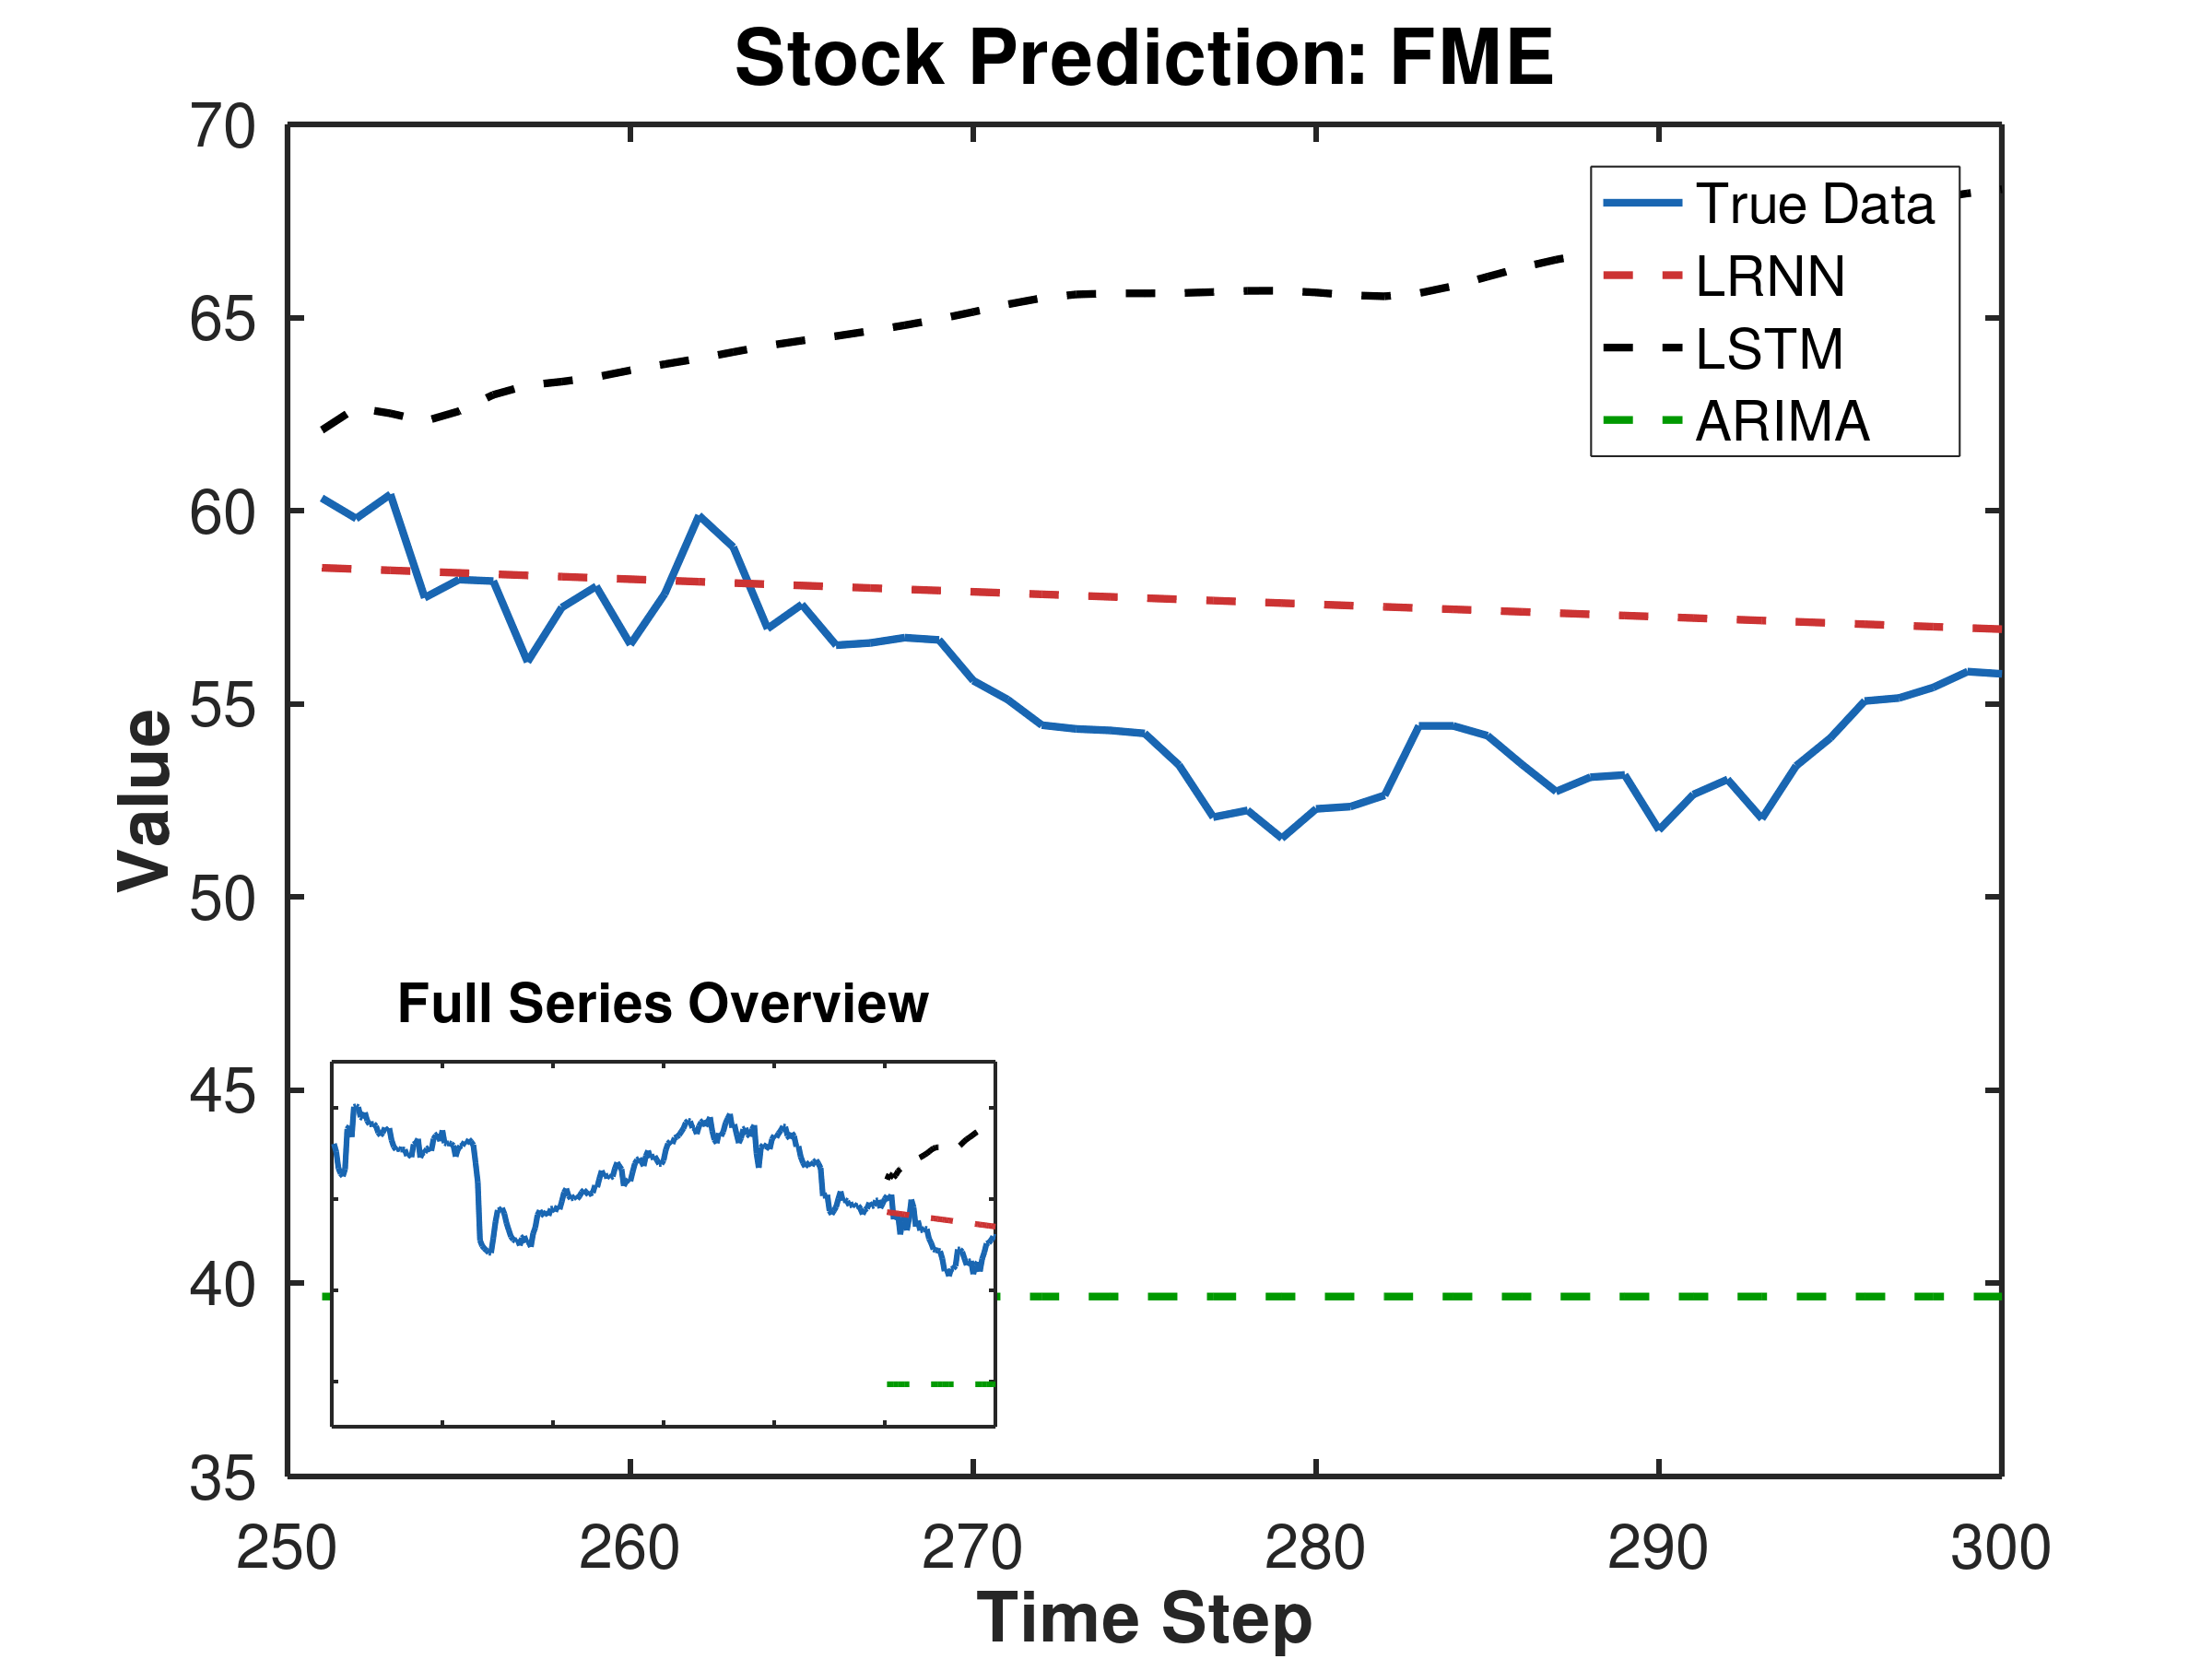
\includegraphics[width=0.65\textwidth]{fig/stock_prediction_fme}
  \caption{Stock price prediction for Fresenius Medical Care (FME.DE) with LRNNs
	(dashed line) and other approaches. The overall performance for all
	approaches often is not much better than the baseline (cf. \cref{dax}).}
  \label{stockfig}
\end{figure}

\begin{table}
\small
\begin{tabular}{l@{ }crcccccc}
\toprule
\multicolumn{2}{c}{DAX member} & \head{mean} & Baseline & ARIMA & ESN & LSTM & \multicolumn{2}{l}{LRNN}\\
name & stock & \head{training} & RMSE & RMSE & RMSE & RMSE & $N$ & RMSE\\ \midrule
Adidas & ADS.DE & 280.8500 & \textbf{0.0554} & 0.0554 & 0.0784 & 0.1162 & 2 & 0.0569\\
Airbus & AIR.DE & 99.6260 & 0.0618 & 0.1070 & 0.0583 & 0.2293 & 2 & \textbf{0.0500}\\
Allianz & ALV.DE & 188.3300 & 0.0252 & 0.0241 & \textbf{0.0199} & 0.0916 & 2 & 0.0503\\
BASF & BAS.DE & 59.9500 & 0.0438 & \textbf{0.0262} & 0.0739 & 0.1218 & 2 & 0.0433\\
Bayer & BAYN.DE & 47.8990 & 0.0414 & 0.0409 & 0.0626 & 0.1027 & 1 & \textbf{0.0350}\\
BMW St & BMW.DE & 72.4980 & 0.0706 & \textbf{0.0706} & 0.0744 & 0.1509 & 11 & 0.0787\\
Brenntag & BNR.DE & 71.4050 & \textbf{0.0544} & 0.0938 & 0.0664 & 0.1162 & 2 & 0.0969\\
Continental & CON.DE & 110.3400 & 0.0518 & \textbf{0.0518} & 0.0803 & 0.2540 & 2 & 0.1918\\
Covestro & COV1.DE & 50.1070 & \textbf{0.0488} & 0.0488 & 0.0564 & 0.1612 & 1 & 0.0609\\
Deutsche Börse & DB1.DE & 135.9100 & 0.0307 & 0.0307 & \textbf{0.0249} & 0.0814 & 1 & 0.0347\\
Deutsche Bank & DBK.DE & 10.0720 & 0.0442 & 0.0442 & \textbf{0.0229} & 0.1794 & 1 & 0.0599\\
Delivery Hero & DHER.DE & 116.7200 & 0.1119 & 0.1040 & 0.1148 & 0.2226 & 3 & \textbf{0.0798}\\
Deutsche Post & DPW.DE & 46.5780 & 0.0487 & 0.0379 & \textbf{0.0369} & 0.1822 & 1 & 0.0549\\
Deutsche Telekom & DTE.DE & 15.5660 & 0.0279 & 0.0279 & 0.0619 & 0.1209 & 2 & \textbf{0.0224}\\
Deutsche Wohnen SE & DWNI.DE & 45.8590 & 0.2410 & 0.2410 & 0.2468 & \textbf{0.1706} & 1 & 0.2589\\
Siemens Energy & ENR.DE & 26.2940 & 0.0457 & 0.0457 & 0.0364 & 0.2212 & 9 & \textbf{0.0349}\\
E.ON & EOAN.DE & 9.0860 & 0.0646 & 0.0646 & 0.0666 & 0.4041 & 1 & \textbf{0.0389}\\
Fresenius Medical Care & FME.DE & 63.4290 & 0.0831 & 0.0842 & 0.0916 & 0.1279 & 1 & \textbf{0.0738}\\
Fresenius & FRE.DE & 38.8670 & 0.1256 & 0.1256 & 0.1560 & 0.1399 & 2 & \textbf{0.1228}\\
HeidelbergCement & HEI.DE & 64.7440 & 0.0504 & \textbf{0.0259} & 0.0708 & 0.1171 & 2 & 0.0912\\
Henkel Vz & HEN3.DE & 84.8720 & 0.0476 & 0.0476 & 0.0328 & 0.1479 & 2 & \textbf{0.0237}\\
HelloFresh & HFG.DE & 71.3430 & 0.1236 & 0.1236 & 0.1241 & 0.3065 & 2 & \textbf{0.1220}\\
Infineon & IFX.DE & 32.8380 & 0.1035 & 0.1029 & 0.1623 & 0.3574 & 1 & \textbf{0.0705}\\
Linde PLC & LIN.DE & 229.9400 & 0.1077 & \textbf{0.0710} & 0.1134 & 0.1803 & 1 & 0.0909\\
Merck KGaA & MRK.DE & 153.7900 & 0.1293 & 0.0826 & \textbf{0.0332} & 0.2156 & 1 & 0.0361\\
MTU Aero Engines & MTX.DE & 198.4500 & \textbf{0.0598} & 0.0600 & 0.1085 & 0.2046 & 2 & 0.0652\\
Münchener Rück & MUV2.DE & 225.1500 & 0.0257 & \textbf{0.0256} & 0.0430 & 0.1276 & 1 & 0.0421\\
Porsche Vz & PAH3.DE & 73.8450 & \textbf{0.0690} & 0.1116 & 0.0920 & 0.1710 & 2 & 0.1188\\
Puma & PUM.DE & 91.3340 & 0.0894 & 0.0887 & 0.0783 & 0.1737 & 1 & \textbf{0.0531}\\
Qiagen & QIA.DE & 42.4940 & 0.0660 & 0.0660 & 0.0810 & 0.1311 & 2 & \textbf{0.0225}\\
RWE & RWE.DE & 31.5540 & 0.0460 & 0.0460 & 0.0805 & 0.1202 & 2 & \textbf{0.0276}\\
SAP & SAP.DE & 110.8400 & 0.0398 & \textbf{0.0398} & 0.0459 & 0.1200 & 2 & 0.0442\\
Siemens Healthineers & SHL.DE & 47.7620 & 0.1057 & 0.0561 & 0.0975 & 0.1898 & 1 & \textbf{0.0328}\\
Siemens & SIE.DE & 127.4800 & 0.0561 & \textbf{0.0354} & 0.0758 & 0.1276 & 2 & 0.0996\\
Sartorius Vz & SRT3.DE & 445.1700 & 0.0676 & 0.0676 & 0.0591 & 0.2400 & 1 & \textbf{0.0463}\\
Symrise & SY1.DE & 108.7900 & 0.1032 & 0.1032 & 0.0893 & 0.1055 & 1 & \textbf{0.0755}\\
Vonovia & VNA.DE & 52.4410 & 0.0714 & 0.0801 & 0.0662 & 0.1222 & 1 & \textbf{0.0593}\\
Volkswagen Vz & VOW3.DE & 177.7200 & \textbf{0.0615} & 0.0615 & 0.1207 & 0.1521 & 2 & 0.1181\\
Zalando & ZAL.DE & 89.9610 & 0.0656 & 0.0656 & 0.1139 & 0.2111 & 2 & \textbf{0.0600}\\
\bottomrule
\end{tabular}
\caption{Evaluation results for all stocks in the DAX existing at least 300
trading days until the end of 2021. The best performing
approach is highlighted by bold face. For LRNNs, the network size $N$ after size
reduction is shown.}
\label{dax}
\end{table}

\section{Conclusions}\label{conclude}

In this paper, we have introduced LRNNs. The major innovation in this work is a
closed-form approach to network size reduction (cf.
\cref{reduce}) that learns both architecture and parameters of linearly activated RNNs.
No backpropagation, gradient-descent, or other iterative procedure with several
epochs is required, and the approach leads to significantly smaller, sparsely
connected, and in many cases even minimal size networks.

We have shown that despite its simplicity of using only linear activation in the
recurrent layer, LRNNs are a powerful approach to model time-dependent functions.
The training procedure only uses standard matrix operations and is thus quite fast.
In contrast to ESNs, also, no washout period is required. Any
function can be approximated directly from its first step, with an arbitrary
start vector (cf. \cref{chad}).
Experiments with reasonably large example and network sizes can be performed
successfully within seconds on standard hardware.
However, if thousands of reservoir neurons are employed, the procedure may
become numerically unstable, at least our Octave implementation. The likelihood
of almost identical eigenvectors and eigenvalues with absolute values greater
than $1$ in the learned transition matrix $W$ is increased then. Nonetheless,
the underlying major problem here seems to be that existing scientific
programming libraries do not calculate the eigenvalues of large matrices
accurately enough. This point needs further investigation.

A particularly interesting application of our approach reducing the network size
is in hardware implementations of neural networks, e.g., for neuromorphic or
reservoir computing~\citep{Mea90,IL+11,LL17}. Neuromorphic computing refers to
new hardware that mimics the functioning of the human brain, and neuromorphic
hardware results from the exploration of unconventional physical substrates
and nonlinear phenomena. Future work shall include improving predictive and
memory capacity of LRNNs -- analyzed for small networks by \citet{Mar17} and to
some extent also by \citet{CW+16} -- taking inspiration from convolutional
networks \citep{GBC16}. Last but not least, other machine learning tasks besides
prediction shall be addressed in more detail, including classification and
reinforcement learning~\citep{SB18,PGL17}.

\acks{%
We would like to thank Chad Clark, Andrew Francis, Rouven Neitzel, Oliver Otto,
Kai Steckhan, Flora Stolzenburg, and Ruben Zilibowitz, as well as several
anonymous referees for helpful discussions
and comments. The research reported in this paper has been supported by the
German Academic Exchange Service (DAAD) by funds of the German Federal Ministry
of Education and Research (BMBF) in the Programmes for Project-Related Personal
Exchange (PPP) under grant no.~57319564 and Universities Australia (UA) in the
Australia-Germany Joint Research Cooperation Scheme within the project
\emph{\underline{De}ep \underline{Co}nceptors for Tempo\underline{r}al
D\underline{at}a M\underline{in}in\underline{g}} (Decorating).
A first short and preliminary version of this paper was presented at the conference
\emph{Cognitive Computing} in Hannover \citep{SMO18}. It received the prize for the
most technologically feasible poster contribution.}

\bibliography{recupred}

\end{document}

